\documentclass[11pt,a4paper]{report}

% Aberstwyth dissertation LaTeX Template
% Authors: Dr. Hannah Dee (hmd1@aber.ac.uk), Neil Taylor (nst@aber.ac.uk)
% This has been adapted from the Leeds Thesis template and the 
% Group Project template for Computer Science in Aberystywth University.
% 
% All comments and suggestions welcome.
%
% Template designed to be used with pdflatex: it may need alteration to
% run with a different LaTeX engine

% To build document on the unix command line, run four commands:
 
% pdflatex dissertation
% bibtex dissertation
% pdflatex dissertation
% pdflatex dissertation

% you will end up with dissertation.pdf 
\usepackage{mmp}

% the following packages are used for citations - You only need to include one. 
%
% Use the cite package if you are using the numeric style (e.g. IEEEannot). 
% Use the natbib package if you are using the author-date style (e.g. authordate2annot). 
% Only use one of these and comment out the other one. 
\usepackage{cite}
%\usepackage{natbib}

% Use the following to selectively exclude chapters
%\includeonly{cover,abstract,acknowledge,declare,chapter1,chapter2}

\begin{document}

% all of the include directives below refer to tex files
% so 
\title{Estimation of Terrain Shape Using a Monocular Vision-based System}

% Your name
\author{Connor Luke Goddard}

% Your email 
\authoremail{clg11}

\degreeschemecode{G400} %e.g. G400 
\degreeschemetitle{MEng Software Engineering} % e.g. Computer Science
\degreetype{MEng}

\modulecode{CS39440} % i.e. CS39440, CC39440, CS39620
\moduletitle{Major Project} % i.e. Major Project or Minor Project

\date{6th March 2012} % i.e. the date of this version of the report

\status{Draft} % Use draft until you create the release version. Then, change this to Release.
\version{1.0}

%The title and name of your supervisor.
\supervisor{Dr. Fr\'ed\'eric Labrosse} 

%The email for your supervisor. 
\supervisoremail{ffl}

\maketitle



 includes cover.tex - to change the content,
% edit the tex file

\pagenumbering{roman}

% This is the front page

\title{Estimation of Terrain Shape Using a Monocular Vision-based System}

% Your name
\author{Connor Luke Goddard}

% Your email 
\authoremail{clg11}

\degreeschemecode{G400} %e.g. G400 
\degreeschemetitle{MEng Software Engineering} % e.g. Computer Science
\degreetype{MEng}

\modulecode{CS39440} % i.e. CS39440, CC39440, CS39620
\moduletitle{Major Project} % i.e. Major Project or Minor Project

\date{6th March 2012} % i.e. the date of this version of the report

\status{Draft} % Use draft until you create the release version. Then, change this to Release.
\version{1.0}

%The title and name of your supervisor.
\supervisor{Dr. Fr\'ed\'eric Labrosse} 

%The email for your supervisor. 
\supervisoremail{ffl}

\maketitle



                        

% Set up page numbering
\pagestyle{empty}

% declarations of originality 
\thispagestyle{empty}

%%%
%%% You must sign the declaration of originality. 
%%%
\begin{center}
    {\LARGE\bf Declaration of originality}
\end{center}

In signing below, I confirm that:

\begin{itemize}
\item{This submission is my own work, except where clearly
indicated.  }

\item{I understand that there are severe penalties for plagiarism 
and other unfair practice, which can lead to loss of marks
or even the withholding of a degree. }
 
\item{I have read the sections on unfair practice in the Students' 
Examinations Handbook and the relevant sections of the 
current Student Handbook of the Department of Computer 
Science.}
 
\item{I understand and agree to abide by the University's
regulations governing these issues.}
\end{itemize}

\vspace{2em}
Signature ............................................................  \\

\vspace{1em}
Date ............................................................ \\

%%% 
%%% We would like to make a selection of final reports available to students that take 
%%% this module in future years. To enable us to do this, we require your consent. You 
%%% are not required that you do this, but if you do give your consent, then we will have 
%%% the option to select yours as one of a number of reports as examples for other 
%%% students. If you would like to give your consent, then please include the following 
%%% text and sign below. If you do not wish to give your consent, please remove this 
%%% from your report. 
%%%
\vspace{1em}
\begin{center}
    {\LARGE\bf Consent to share this work}
\end{center}

In signing below, I hereby agree to this dissertation being made available to other
students and academic staff of the Aberystwyth Computer Science Department.  

\vspace{2em}
Signature ............................................................  \\

\vspace{1em}
Date ............................................................ \\

\vspace{3em}

\begin{center}
    {\LARGE\bf Ethics Form Application Number}
    
% You need to replace NUMBER with the number you are emailed when you complete your 
% ethics application.     
The Ethics Form Application Number for this project is: 841. 
\end{center}

\vspace{2em}

\begin{center}
    {\LARGE\bf Student Number}

% Change this so that you use the barcode image that you have downloaded.
% We don't mind if you choose to scale this to a minimum of 50% of the original size. 
% We will be scanning this as part of the process to manage your hand in. Make sure 
% that you use the barcode image we have provided, which contains your individual number. 

\includegraphics[scale=0.6]{Images/clg11-barcode.png}
\end{center}


               

\thispagestyle{empty}

\begin{center}
    {\LARGE\bf Acknowledgements}
\end{center}

I wish to thank my project supervisor, Dr. Fr\'{e}d\'{e}ric Labrosse for all of his guidance and vast levels of patience he gave in spades throughout the duration of the project. Many of the ideas presented in this paper were originally suggested by Fred, before being developed further through a combined effort. 

I also wish to thank all of my family for their continued support during my academic studies, and a particular thank you to my partner Sioned, who without I certainly would not have achieved all that I have to this point. % Acknowledgements
\thispagestyle{empty}

\begin{center}
    {\LARGE\bf Abstract}
\end{center}

Include an abstract for your project. This should be no more than 300 words.
                 % Abstract

\pagenumbering{roman}
\pagestyle{fancy}
\fancyhead{}
\fancyfoot[C]{\thepage}
\renewcommand{\headrulewidth}{0 pt}
\renewcommand{\chaptermark}[1]{\markboth{#1}{}}

\tableofcontents   
\newpage
\listoffigures
\newpage 
\listoftables
\newpage

% Set up page numbering
\pagenumbering{arabic}

\title{Estimation of Terrain Shape Using a Monocular Vision-based System}

\setchapterheaderfooter

% include the chapters
\chapter{Background \& Objectives}

%This section should discuss your preparation for the project, including background reading, your analysis of the problem and the process or method you have followed to help structure your work.  It is likely that you will reuse part of your outline project specification, but at this point in the project you should have more to talk about. 
%
%\textbf{Note}: 
%
%\begin{itemize}
%   \item All of the sections and text in this example are for illustration purposes. The main Chapters are a good starting point, but the content and actual sections that you include are likely to be different.
%   
%   \item Look at the document on the Structure of the Final Report for additional guidance. 
%   
%\end {itemize}
%
%\section{Background}
%What was your background preparation for the project? What similar systems or research techniques did you assess? What was your motivation and interest in this project? 
%
%\section{Analysis}
%Taking into account the problem and what you learned from the background work, what was your analysis of the problem? How did your analysis help to decompose the problem into the main tasks that you would undertake? Were there alternative approaches? Why did you choose one approach compared to the alternatives? 
%
%There should be a clear statement of the research questions, which you will evaluate at the end of the work. 
%
%In most cases, the agreed objectives or requirements will be the result of a compromise between what would ideally have been produced and what was felt to be possible in the time available. A discussion of the process of arriving at the final list is usually appropriate.
%
%\section{Research Method}
%You need to describe briefly the life cycle model or research method that you used. You do not need to write about all of the different process models that you are aware of. Focus on the process model or research method that you have used. It is possible that you needed to adapt an existing method to suit your project; clearly identify what you used and how you adapted it for your needs.

\section{Background}

\subsection{Introduction}

The ability to decide between one or more alternate choices is a complex skill that as humans, we possess but rarely consciously observe. As human beings, we are expected to make decisions both large and small as part of everyday life, but . While most decisions will have typically little impact requiring almost unnoticeable levels of thought (e.g. \textit{``do I have peas or beans tonight with dinner?"}), others that could have potentially life-changing consequences (e.g. \textit{"do I take this new job or not?"}) will force an individual to consider much more closely.

For a human faced with making such decisions, identifying which out of a number of possible choices constitutes the ``right" decision is often regarded as a challenging and highly subjective task. %Each decision that a person makes will vary based upon their individual characteristics, which as a consequence can often result in contrasting decisions being taken in response to the same situation.% 
Before settling on a final decision, an individual will typically identify and evaluate all possible choices by considering each upon a weighting of merit \cite{rational-decision-model}. While variations in weighting between specific individuals can cause different decision outcomes, an important realisation comes from the understanding that all considerations made by an individual rely on their \textit{trust} in the accuracy and truth of information gathered during the identification and comparison of these alternative choices.

 In considering any kind of autonomous system that is expected to make unattended decisions, a crucial yet not always obvious aspect is a reliance upon this idea of \textit{trust}. In the same way as observed in humans, a system will typically depend upon underlying information from which it can assess that the final decision when made is most appropriate for a given situation.
 
 This information may be obtained from a variety of sources, ranging from raw sensor data up to the output of a sophisticated high-level algorithm. While the type and source of information may vary wildly from system-to-system, the underlying notion that at the time of making the final decision this information can, in one form or another, be \textit{trusted} to provide a reliable and accurate representation of the actual situation remains exactly the same. 
 
Given the importance of the relationship between reliable information and correct decision making, a major challenge within the field of autonomous robotics is maximising both the accuracy of input data, and the robustness of systems used to verify such accuracy.

  Accurate and efficient navigation plays a crucial role in allowing robots that require autonomous motion capabilities to make safe, yet objective decisions on how best to traverse from a starting position to a target position. This idea becomes evermore important when it is considered that a key use case for robotic systems typically involves the undertaking of tasks within environments deemed unfeasible or unsafe for humans to complete themselves. Observing examples of tasks where autonomous robots are expected to operate in particularly harsh environments, including bomb disposal \cite{bomb-disposal} and planetary exploration \cite{planet-explore}, it becomes clear that the ability to perform safe and robust navigation is vital to the survival of both mission and device.

As a problem-space, autonomous navigation can be decomposed into two key areas of focus; one of \textit{reactive} navigation, and the other of \textit{deliberative} navigation. Reactive, or local navigation is concerned with controlling the path of the robot through the immediate surrounding area, focussing in particular on the safe traversal around potentially dangerous terrain hazards including obstacles, steep slopes and precipices. In contrast, deliberative or global navigation is tasked with planning the ``high-level" path that a robot will follow in order to reach its destination. As a consequence, deliberative navigation tends to adopt a greater level of focus on calculating the most \textit{optimal} path through the environment over necessarily the one that is ``safest" for the robot. Traditionally within autonomous navigation systems, feedback from both the reactive and deliberative components is combined in order to arrive at final path that balances both safety and objectivity \cite{mer-rover}. 

A vital contributor to the success of reactive navigation and therefore to the overall survival of an autonomous robot is the identification and subsequent avoidance of obstacles. As a result, the development of accurate and robust obstacle detection systems is a keen and well-explored area of robotics research, with a variety of approaches now available adopting many types of sensor including sonar \cite{sonar-sensor} and laser scanning \cite{laser-sensor}. An alternative approach that has enjoyed increasingly greater research focus over the past decade is that of vision-based obstacle avoidance. This involves the analysis of images captured from one or more digital cameras in order to detect and classify possible dangers currently situated within the robot's field of view. 

Cameras are becoming an increasingly favourable sensor for use on robotic systems, due primarily to the impressive variety and quantity of potential data that can be captured \textit{simultaneously} from a single device. They are also one of few sensors that have experienced a consistent reduction in price over the past decade \cite{campbell}, making them viable for many types of project application and budget. 

\subsection{Computer Vision Principles}

\subsection{Related Work}

A large variety of solutions to vision-based navigation and obstacle avoidance have previously been published, with the majority proposing new or improved approaches to combining ``standard" computer-vision techniques including optical flow, feature tracking and template patch tracking with a variety of hardware configurations including monocular systems, stereo cameras and vision/3D hybrid systems. Typically, these solutions either strive to improve on previously published performance results, or to focus on the avoidance of specific types of obstacle (e.g. precipice or animal detection). 

%From investigating existing research conducted in the area of visual-based navigation and obstacle avoidance, it is possible to identify and compare potential benefits and challenges between various approaches that will in turn feed into future design decisions.

The first approach to be noted is that of the work of Campbell \textit{et al} \cite{campbell} in which the authors propose a system for estimating the change in position and rotation of a robot using information obtained solely via a single consumer-grade colour camera. The approach describes the use of feature-based tracking to estimate the optical flow-field between subsequent video frames, before taking these optical flow vectors currently corresponding to image coordinates, and back-projecting them onto a ``robot-centred" coordinate system to establish the incremental `real world' translation and rotation of the robot over a given time period. The detection and subsequent tracking of matching features between captured frames is provided via the \textit{OpenCV} library implementation of the Lucas and Kanade algorithm \cite{opencv-lucas-kanade-features}. 

Once gathered, these correspondences between features (i.e. optical flow vectors) are filtered to help remove outliers caused by matching error or occlusion. The criteria used for this filtering process focusses on verifying a smooth straight-line motion of same features between subsequent frames. It is reported that concentrating on the movement history of features across a subset of previous frames can provide a robust defence against outliers. This is because by definition, an outlier would typically be expected to be found outside of the projected straight-line trajectory of the mis-matched feature, thereby causing the motion behaviour of this feature to suddenly become erratic. Through the use of this filtering technique in conjunction with the correction of perspective distortion via calibration, the authors report they are able to allow for a wider, and potentially lower quality range of features to be initially detected in order to ensure adequate coverage of the entire image scene. 

In the final stage of the process proposed in \cite{campbell}, the current frame is sectioned into regions representing the ``sky" and ``ground" individually, from within which the observed optical flow vectors are used to calculate an estimation of the robot's incremental rotation and translation respectively.

%The authors report that this implementation provides a more efficient and robust version of the original algorithm proposed by Lucas and Kanade \cite{lucas-kanade-features}. Upon further investigation this improvement appears to be attributed to the proposal published by Bouguet \cite{j-bouguet} in which the author combines a multi-scale pyramidal representation of an image with the existing Lucas-Kanade algorithm. This approach can help to provide both greater accuracy, by locating features that may have moved distances greater than the current window size, while also improving efficiency by means of reducing the size of the search area within higher resolution versions of an image, by first localising the general target area within lower resolution versions that are less computationally expensive to search. 

Of particular interest from the work of Campbell \textit{et al} \cite{campbell} is an approach described for detecting environment hazards solely via the exploitation of the optical flow field. The idea proposed bases itself around the observed discontinuities caused to the optical flow field by scene objects that appear at a different observed depth to camera than the ``normal terrain". In the paper this behaviour is described as a violation of the ``planar world hypothesis", with objects closer to the camera than the ground causing a positive violation, and objects at a greater depth to the camera relative to the ground causing a negative violation. As a consequence, the authors discuss how owing to the effects of motion parallax, it is possible to observe clear differences between subsequent frames in the displacement of scene objects demonstrating either a positive, negative or no violation. This in turn maps onto discontinuities observed in the optical flow field, with objects that move significantly closer to the camera relative to the ground demonstrating longer optical flow vectors, and objects further away from the camera demonstrating the opposite. Given the use of such a seemingly `simple' metric as the proportional length of optical flow vectors, this approach appears to provide positive results, with the authors describing how in practice their system was able to ``detect precipices as near as 3cm". 

An alternative approach proposed by Low and Wyeth \cite{low-wyeth} involves combining sparse feature detection with appearance-based matching in order to track corresponding features between video frames. Firstly, initial features are detected using the same Shi and Tomasi corner detector \cite{shi-tomasi-good-features-to-track} as used in the approach devised by Campbell \textit{et al} \cite{low-wyeth}. 

%This detector is almost identical to the original Harris corner detector \cite{harris-corner} from which it is based, with the only main difference focussing on a change in the use of Eigenvalues to score and classify if an image region should be identified as a corner or not. This slight modification was demonstrated by Shi and Tomasi to provide a greater level of tracking stability and robustness in comparison to the original Harris corner detector \cite{shi-tomasi-good-features-to-track}, and as a result is typically preferred over the original detector proposed by Harris and Stephens. 

Once suitable features have been identified using corner detection, the authors then chose to utilise an appearance-based template matching technique to try and match corresponding windows of neighbouring pixels between subsequent images around each of the detected features. This contrasts with the work of Campbell \textit{et al} \cite{campbell} who instead adopt an entirely feature-based approach to matching corresponding portions of subsequent images. Using the template matching function provided by the \textit{OpenCV} library, the authors describe how a variety of appearance-based matching metrics could easy be evaluated via a simple modification to this function. The authors go on to report how they finally settled on the use of Normalised Cross Correlation as the matching metric, owing primarily to its improved robustness to lighting changes and simple score thresholding range of between 0 and 1, with 1 indicating a perfect match. 

Once obtained, optical flow information is converted to more useful range data using a method known as `Time-to-Contact'. With this approach, it is possible to represent distance to a target as a unit of time \cite{alenya}, and itself is based heavily upon biological mechanisms identified as responsible for providing the correct timing of actions and motion within the brain of humans and birds \cite{lee-young}. Other examples of the use of Time-to-Contact within vision-based systems involving obstacle detection are available in \cite{alenya}, \cite{sagrebin} and \cite{thomas}.

%Contrasting with the more ``ad-hoc" approach adopted by Campbell \textit{et al}, Low and Wyeth choose to generate a map that represents obstacle range information in order to support the detection of obstacles via the analysis of angular range output. 

A major challenge relating to the use of optical flow methods for obstacle detection, and one discussed in the work of both Low and Wyeth \cite{low-wyeth}, and Campbell \textit{et al} \cite{low-wyeth} is the effect that disturbances in rotation (deliberate or otherwise) can cause on the observed optical flow vectors of features. While both papers propose alternative methods for removing the effects of rotation (the use of an Inertial Measurement Unit gyroscope in the case of Low and Wyeth, and a calibrated cylindrical coordinate model in the case of Campbell \textit{et al}), both appear to agree that rotational movement should be accounted separately to translational movement in order to ensure accurate results are obtained from the optical flow field. 

Ulrich and Nourbakhsh \cite{ulrich-nourbakhsh} present an altogether different approach to vision-based obstacle detection. Rather than scrutinising differences in motion behaviour of scene objects, the authors instead focus on comparing differences in colour between the ground and other objects in the robot's field of view. Ulrich and Nourbakhsh argue that using colour as a detection metric for obstacles can prove to be less computationally expensive than ``range-based" obstacle detection methods like optical flow or stereo vision, and in certain cases, have also shown to be more accurate and reliable - particularly in cases involving the detection of small or flat objects close the ground or where a system needs to be able to differentiate between terrain surfaces. 

A key aspect from the Ulrich and Nourbakhsh paper provides details on how their system handles the effects caused by changes in illumination. In their solution to this well-known issue within computer vision, the authors discuss the use of an alternative colour space to RGB for representing input images that allows for the undesired effects caused by changes in illumination between subsequent frames to be negated. By converting images to use the `Hue-Saturation-Intensity' colour space, the actual colour of objects within the image (represented by the Hue and Saturation channels) become less sensitive to changes in brightness (represented by the Intensity channel). As well as providing greater resistance to illumination changes, using a colour space that separates colour from brightness also provided an easier platform from which the authors could further remove noise via channel thresholding \cite{ulrich-nourbakhsh}. 

As part of a survey conducted by Perveen \textit{et al} \cite{perveen} into various methodologies and applications of appearance-based template matching, the authors discuss details of two ``advanced methods" of template matching algorithms that they report can improve both reliability and efficiency when faced with tackling specific pattern-matching tasks. 

 In their report Perveen \textit{et al} first describe how ``Grayscale-based template matching", an enhanced approach to traditional template matching methods, can be shown to support the successful appearance-based detection of objects whose observed appearance may have changed between consecutive images as a result of rotational effects. 
 
 Invariance to object rotation is well-defined issue, and has been an area of keen research interest and progress over recent years. While a number of solutions now exist for providing resilience to differences in the rotation of objects between captured images\cite{sift}, in the majority of cases these solutions are only applicable to methods based upon the use of feature descriptors for the detection and tracking of objects rather than use of their appearance. It is this dependency upon the explicit appearance of objects required by appearance-based matching methods that can make the subsequent matching of objects particularly difficult, given the assumption that for most objects, even a slight rotation could cause its \textit{appearance} to change considerably, thereby resulting in a failure to find a match in cases where an explicit pattern representing an object's appearance is used as a primary metric for similarity equality \cite{find-citation}. 
 
 The authors attribute the apparent robustness to rotational changes provided by Grayscale-based template matching to the use of multiple pyramid structures (traditionally providing support for scale invariance \cite{lowe}), where each structure represents an alternative orientation of the target pattern. While traditionally, such structures are used to help support invariance to scale, once combined they can provide a complete representation of the target pattern under all possible orientations. When subsequently passed to an appearance-based detector, this approach can dramatically improve the chances of a pattern being relocated in the current image, even after potentially experiencing a significant rotational transformation \cite{perveen}. Additional work published in \cite{kim} discusses improvements to the efficiency of this approach by removing pixels deemed unlikely to ever match the target pattern. 
 
 The second 
 
 


\subsection{Project Overview}

Making use of recent advances in camera technology with appropriate computer vision techniques, this project aims to perform a viability study into the use of appearance-based pattern matching and optical flow analysis to provide an estimation into the general ``shape" of the current terrain, while also supporting the detection of obstacles in the path of a mobile robot. 

Through this system, it should be possible to identify the presence of both positive, and negative obstacles (e.g. rocks and pits respectively), providing a reasonable indication of their general size and location.

In addition, it is predicted that such a system will also be able to provide an estimation of the speed and change in rotation/orientation of the robot as it traverses along a path. These will be calculated as by-products of the terrain inference mechanism, and could form part of a larger visual odometry system.

While the primary aims of the proposed project are research-focussed, the ultimate goal of the project will be to implement the system onto a working mobile robot, such as the `IDRIS' all-terrain wheeled robot currently in use by the Aberystwyth University Computer Science department.

\subsection{Motivation}



\section{Analysis}


\subsection{Overview}

\subsection{Research Aims}

\subsection{Design Decisions}

\subsubsection{Feature Matching}

\subsubsection{Development Environment}

\section{Research Methodology}

\subsection{Overview}

\subsection{Development Process}

\subsection{Testing}

\section{Project Working Hypothesis}




%\addcontentsline{toc}{chapter}{Development Process}
\chapter{Experiment Methods}
%
%This section should discuss the overall hypothesis being tested and justify the approach selected in the context of the research area.  Describe the experiment design that has been selected and how measurements and comparisons of results are to be made. 
%
%You should concentrate on the more important aspects of the method. Present an overview before going into detail. As well as describing the methods adopted, discuss other approaches that were considered. You might also discuss areas that you had to revise after some investigation. 
%
%You should also identify any support tools that you used. You should discuss your choice of implementation tools or simulation tools. For any code that you have written, you can talk about languages and related tools. For any simulation and analysis tools, identify the tools and how they are used on the project. 
%
%If your project includes some engineering (hardware, software, firmware, or a mixture) to support the experiments, include details in your report about your design and implementation. You should discuss with your supervisor whether it is better to include a different top-level section to describe any engineering work.  

This chapter aims to provide a discussion into the experiments implemented with respect to the investigation detailed in Chapter 1, providing an emphasis on the approaches that were adopted and the resulting actions of handling issues encountered.

The results subsequently collected from these experiments are presented in the Chapter 3.

\section{Collection of Appropriate Test Data}

Prior to beginning the implementation of any experiments, it was first necessary to identify and collect sets of sample images which would accurately represent the types of input expected upon the deployment of a completed system into a live scenario. 

\subsection{Image Data Requirements}

As discussed previously in Section \ref{assumptions}, for the purposes of simplifying the \textit{primary aims} presented in the working hypothesis, the assumption was drawn that at least in early stages of investigation, the system would make exclusive use of images captured from a single camera positioned to face in front of the robot that was also limited to moving in the same direction as the camera (i.e. forward-motion only).

Therefore when identifying appropriate test data for use in experiments, a the following characteristics were considered:

\begin{itemize}
	\item The images must provide a reasonable field of view of the current scene both above and below the horizon line (i.e it was important to capture objects within the scene located both far away and close to the camera)
	\item The images must show the act of forward translation through the current environment. This would be most obvious through the observation of a vertical displacement in the negative direction (i.e. downwards) visible in features located along the ground plane.
	\item The images must not show forward translation as horizontal movement across the image plane (i.e. no images captured from cameras looking out from the side of a robot moving in a forwards direction).
	\item The images must be of a size and quality reasonably expected of a standard ``point-and-shoot" consumer-grade camera.
	\item The images must have been originally captured in colour, using the ``default" colour space supported by the camera (typically this would be RGB for standard consumer-grade camera).
	 \item The images should demonstrate minimal change in rotation or pitch (i.e. should be taken across a flat surface), and should be 
\end{itemize}

In addition to these ``baseline" requirements, additional requirements were also defined with the intention for use within specific experiments focussing on the identification of particular aspects in motion behaviour. These secondary requirements were very much intended to be used on an ``as needed" basis and came with the possibility of the opposite statement to the ones detailed below being desired in certain situations:

\begin{itemize}
	\item The images should demonstrate minimal rotational motion (i.e. no examples of the robot turning to change direction)
	\item The images should capture terrain that is predominately flat and free of major obstacles both positive (e.g. rocks) and negative (e.g. pits).
\end{itemize}

Unfortunately due to time constraints, some the planned experiments could not be completed within the scope of the major project, and as a consequence of this, not all examples of images meeting every one these requirements were actually captured. However, it was still important to define these requirements before beginning any experimentation and given more time, would still prove to be valid.

\subsection{Existing Datasets}

At the beginning of the project, some time was initially devoted to searching for any existing datasets that could provide suitable imagery. One of the main advantages to using existing datasets, is that typically other previous projects have already had the opportunity to verify that the data is both accurate, and provides a sufficient level of variability that proves crucial in testing the robustness of the systems that make use them as part of their evaluation.

In the majority of cases, existing datasets also come pre-packaged with appropriately verified ground truth data, thereby preventing the need for projects that subsequently chose to use them having to produce their own ground truth results, consequently saving on both time and resources.

While a number of previously published datasets were found to be available \cite{ucl-dataset}, \cite{baker-dataset}, \cite{mpi-dataset}, unfortunately none were found to be suitable in relation to the requirements detailed in the previous sub-section.   

\subsection{Manual Datasets}

Following the lack of appropriate existing datasets with the field, it was deemed necessary that bespoke datasets would instead have to be created manually. While in the short term this meant an increased work load, it also presented the opportunity to capture datasets that would could specifically meet the needs of the investigation and its experiments.

\subsubsection{Camera Rig Setup}

In the pursuit of capturing image datasets, a wide range of approaches could have potentially been adopted. One initial idea considered requesting the use of one of several `Pioneer' robots owned by the Computer Science department at Aberystwyth University. By rigidly mounting a camera to the front of one of these small wheeled robots, and remotely instructing it to move forward by a set distance before manually triggering the camera, it would be achievable to capture a collection of images in which each demonstrated an equal level of displacement between that and the next image. 

As part of a particularly elaborate setup, it would have perhaps been feasible to provide an interface to the mounted camera (perhaps via USB or serial) before programming the Pioneer robot into automatically capturing images at set intervals, while following a pre-determined path through the environment (making use of the on-board sonar and odometry capabilities). 

While these approaches would certainly provide an ample solution, following a discussion with the project supervisor, it was deemed that, at such an early stage in an investigation that was already limited in time remaining, efforts would be better spent focussing on conducting actual research, as opposed to the collection of test data.

Nevertheless, a means of manually capturing image datasets was still required. As such, the decision was taken to adopt a much more `simplified' approach, that in exchange for greater manual involvement, could consequently be brought into service within a vastly shorter timeframe. 

Compared to the use of the robot, this approach was certainly less `sophisticated' in terms of its setup, consisting only of:

\begin{itemize}
	\item Two cardboard boxes (one rectangular and one angled);
	\item A consumer-grade ``point-and-shoot" camera (Panasonic Lumix DMC-FS18);
	\item A standard 30cm ruler;
	\item A standard spirit level;
\end{itemize}

However, as well as being quick to initially build, this setup would go on to prove to be a lot more portable and a great deal cheaper to modify and fix than one of the Pioneer robots. 

The method behind the use of the `homemade' camera rig was also simple in design, however this was regarded as favourable given that it solely relied on manual involvement where human error subsequently becomes one of the biggest issues to face. Figure \ref{} below details the method outline: 

% ADD FIGURE SHOWING FLOW CHART FOR METHOD (STEP 1 - GO TO START POSITION)...

While one of the aims of the investigation hypothesis was to avoid the need for calibration of the camera, it was decided that in the interests of good experiment practice, measurements regarding the physical setup of the camera rig should be taken in case of future need. The measurements that were taken matched those taken by in the work by Campbell \textit{et al.}  \cite{campbell}, where the authors detailed their physical setup shown in Figure \ref{}:
\\
\\
\\
\\
\\
where $h$ refers to the height of the camera from the ground, and $d$ refers to the distance between the camera lens and the intersection with the ground plane. 

In order to calculate $d$, a target $T$ was first lined up on the ground such that it became positioned in the centre of the camera's viewfinder (Figure \ref{}). Next, the height $h$ was measured, along with the distance between the position of the target $T$, and the position $L$ where the front of the camera lens intersected vertically with the floor. Finally, Pythagorus' theorem was adopted to calculate the length of $d$:

$$ a^2 = \sqrt{b^2 + c^2} $$

It was also possible to calculate the angle of the camera towards the ground plane by using simple trigonometry to taking the inverse tangent \cite{campbell}:

$$ maths $$

\subsubsection{Environments}

\section{Establishment of Ground Truth}

\section{Test Harness}

\section{Template Matching (Full-width Patches) - Non Scaled}

\subsection{Perspective Distortion Calibration Tool}

\subsection{Calibration Evaluation Images}

\section{Template Matching (Full-width Patches) - Scaled}

\section{Investigating Alternative Existing Methods}

\subsection{Feature-based matching techniques}

\subsection{Edge-based matching techniques}




\chapter{Results and Conclusions}

%This section should discuss issues you encountered as you tried to implement your experiments. What were the results of running the experiments? What conclusions can you draw from these results? 
%
%During the work, you might have found that elements of your experiments were unnecessary or overly complex; perhaps third party libraries were available that simplified some of the functions that you intended to implement. If things were easier in some areas, then how did you adapt your project to take account of your findings?
%
%It is more likely that things were more complex than you first thought. In particular, were there any problems or difficulties that you found during implementation that you had to address? Did such problems simply delay you or were they more significant? 
%
%If you had multiple experiments to run, it may be sensible to discuss each experiment in separate sections. 

This chapter presents the key results from the three primary experiments conducted under the investigation for this project. 


\section{Investigation Results}

\clearpage
\subsection{Experiment 1: Template Matching (Overlapping Small Patches)}

\subsubsection{Dataset 1: Living Room Carpet (Indoors)}

\begin{figure}[ht!]
\centering
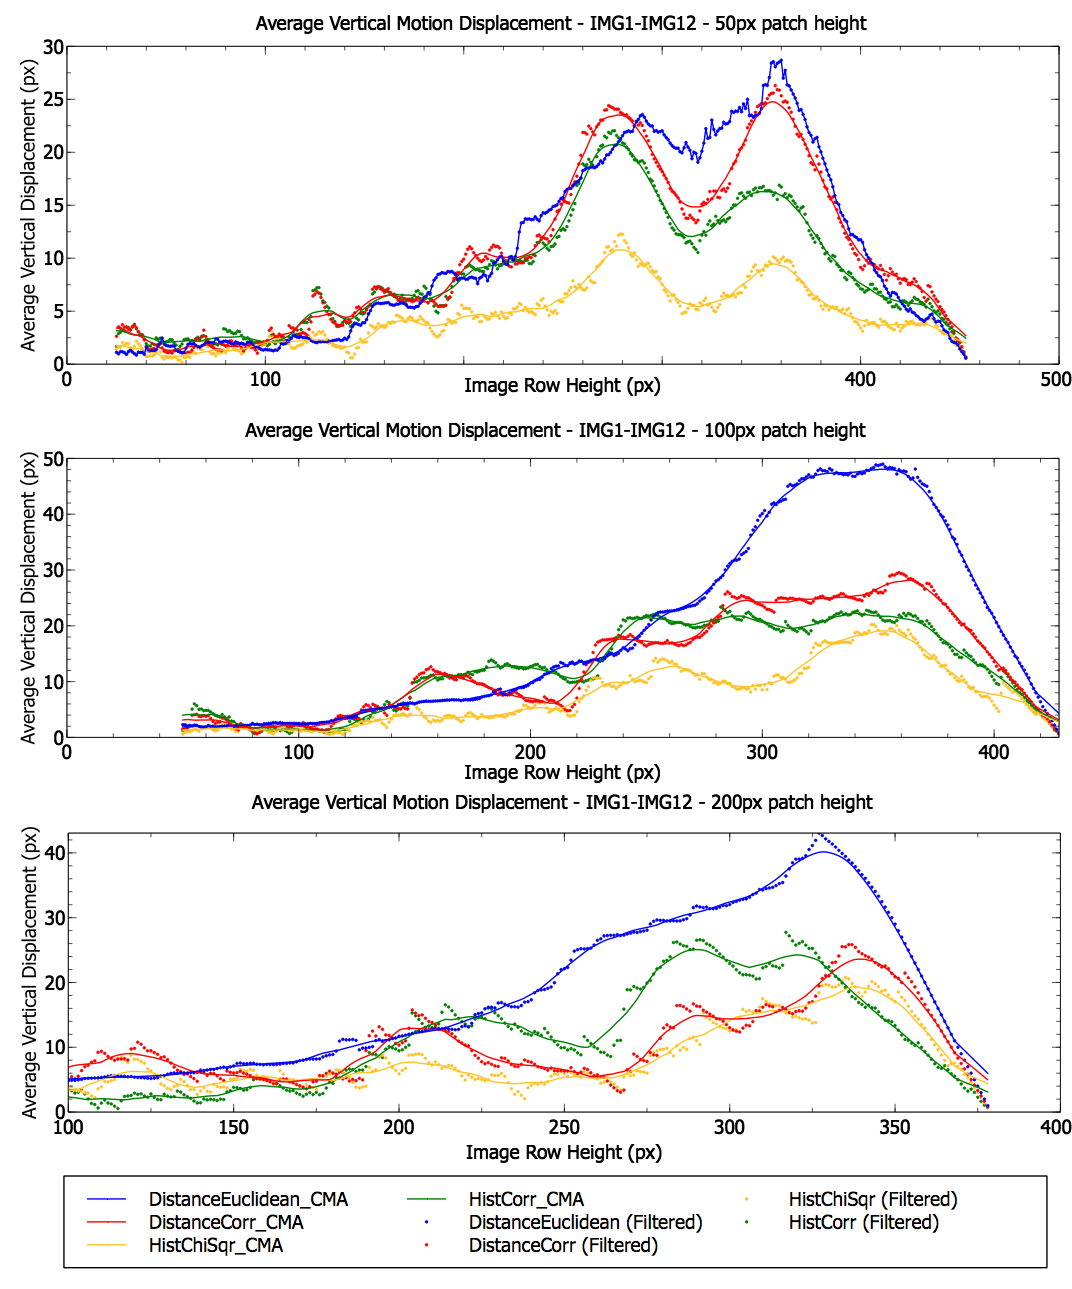
\includegraphics[scale=0.4]{images/results/ex1_results_flat_10cm}
\caption{Average vertical motion displacement models across all images within ``living room carpet" dataset running \textit{non-exhaustive} localised search. Graph 1 (Top) - Overlapping patches of 50px-square; Graph 2 (Middle) Overlapping patches of 100px-square; Graph 3 (Bottom) Overlapping patches of 200px-square. Solid line indicates centred moving average (10-pixel interval) calculated from filtered results for each image similarity metric.}
\label{fig:ex1_1_1}
\end{figure}

The results within Figure \ref{fig:ex1_1_1} indicate an increase between the position of matched features along the vertical axis of the image, and the subsequent vertical displacement that is demonstrated between two consecutive images. While this trend is visible across all three patch sizes, the maximum displacement is recorded using the 100px patch size. Out of the four similarity metrics, Euclidean Distance appears to show the best performance across all of the  patch sizes.

\clearpage
\subsubsection{Dataset 2: Brick-Paved Road (Outside)}

\begin{figure}[ht!]
\centering
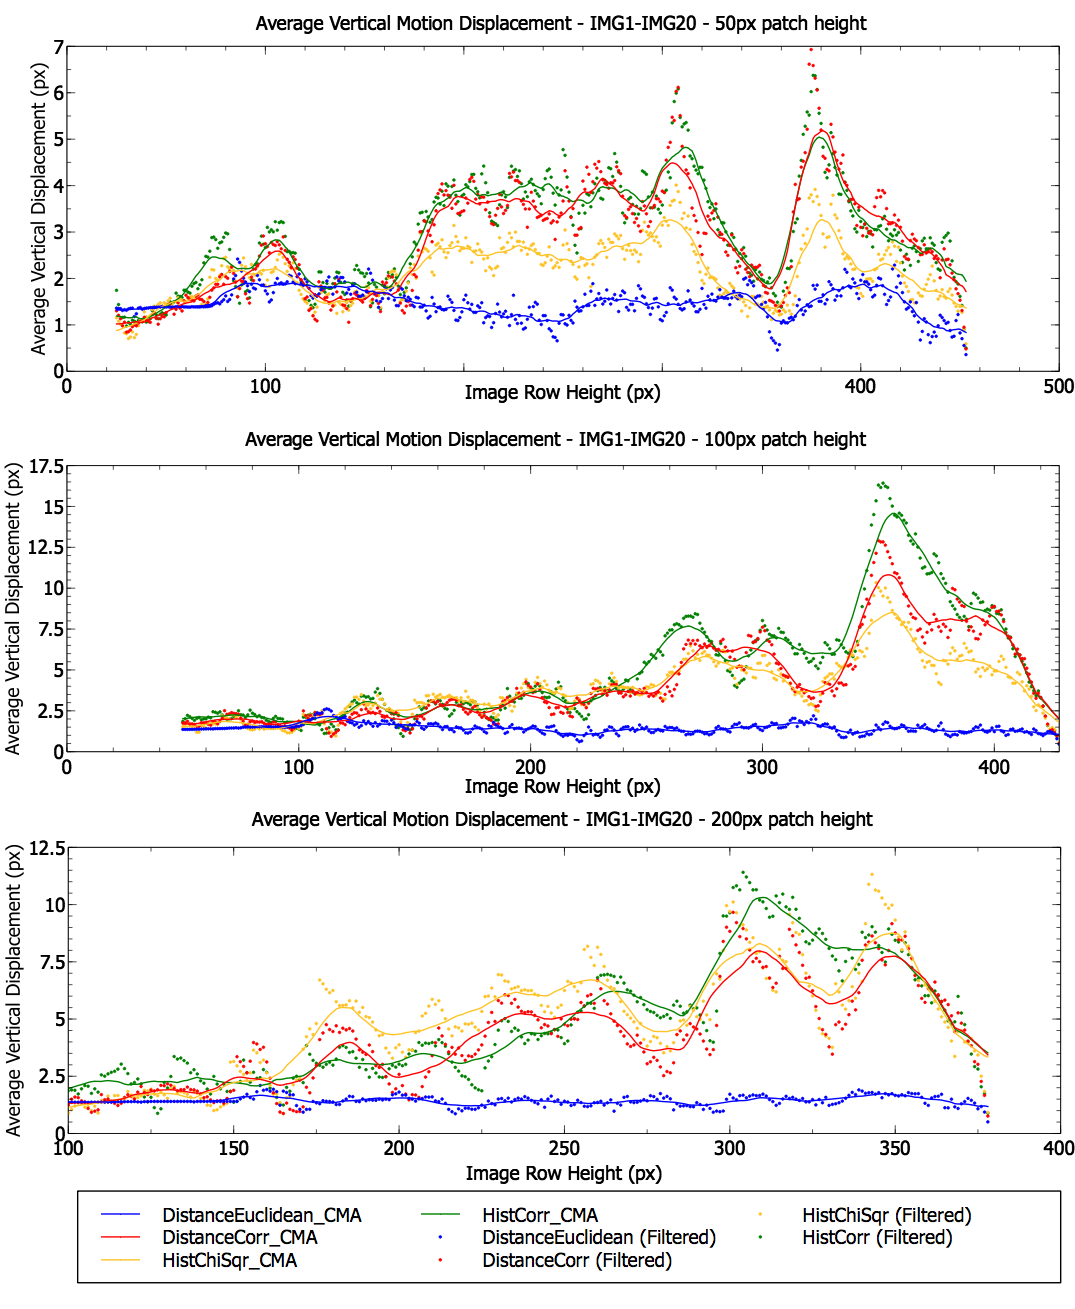
\includegraphics[scale=0.4]{images/results/ex1_results_outside_10cm}
\caption{Average vertical motion displacement models across all images within ``brick-paved road" dataset running \textit{non-exhaustive} localised search. Graph 1 (Top) - Overlapping patches of 50px-square; Graph 2 (Middle) Overlapping patches of 100px-square; Graph 3 (Bottom) Overlapping patches of 200px-square. Solid line indicates centred moving average (10-pixel interval) calculated from filtered results for each appearance-based template matching similarity metric.}
\label{fig:ex1_1_2}
\end{figure}

For dataset two, the results show while there does still appear to be an overall positive correlation shown in Figure \ref{fig:ex1_1_1}, across all three patch sizes it is much weaker and with a significant level of distortion. While the two histogram-based similarity measures and Normalised Cross-Correlation all provided similar results, the Euclidean Distance appears to consistently fail in identifying any significant displacement. Interestingly, Graph 1 shows how all three of the better-performing similarity measures suddenly report a dip in displacement at around row 300, before returning again just before row 400. (\ref{fig:ex1_1_2}).

\clearpage
\subsubsection{Dataset 3: Asian Rug (Indoors)}

\begin{figure}[ht!]
\centering
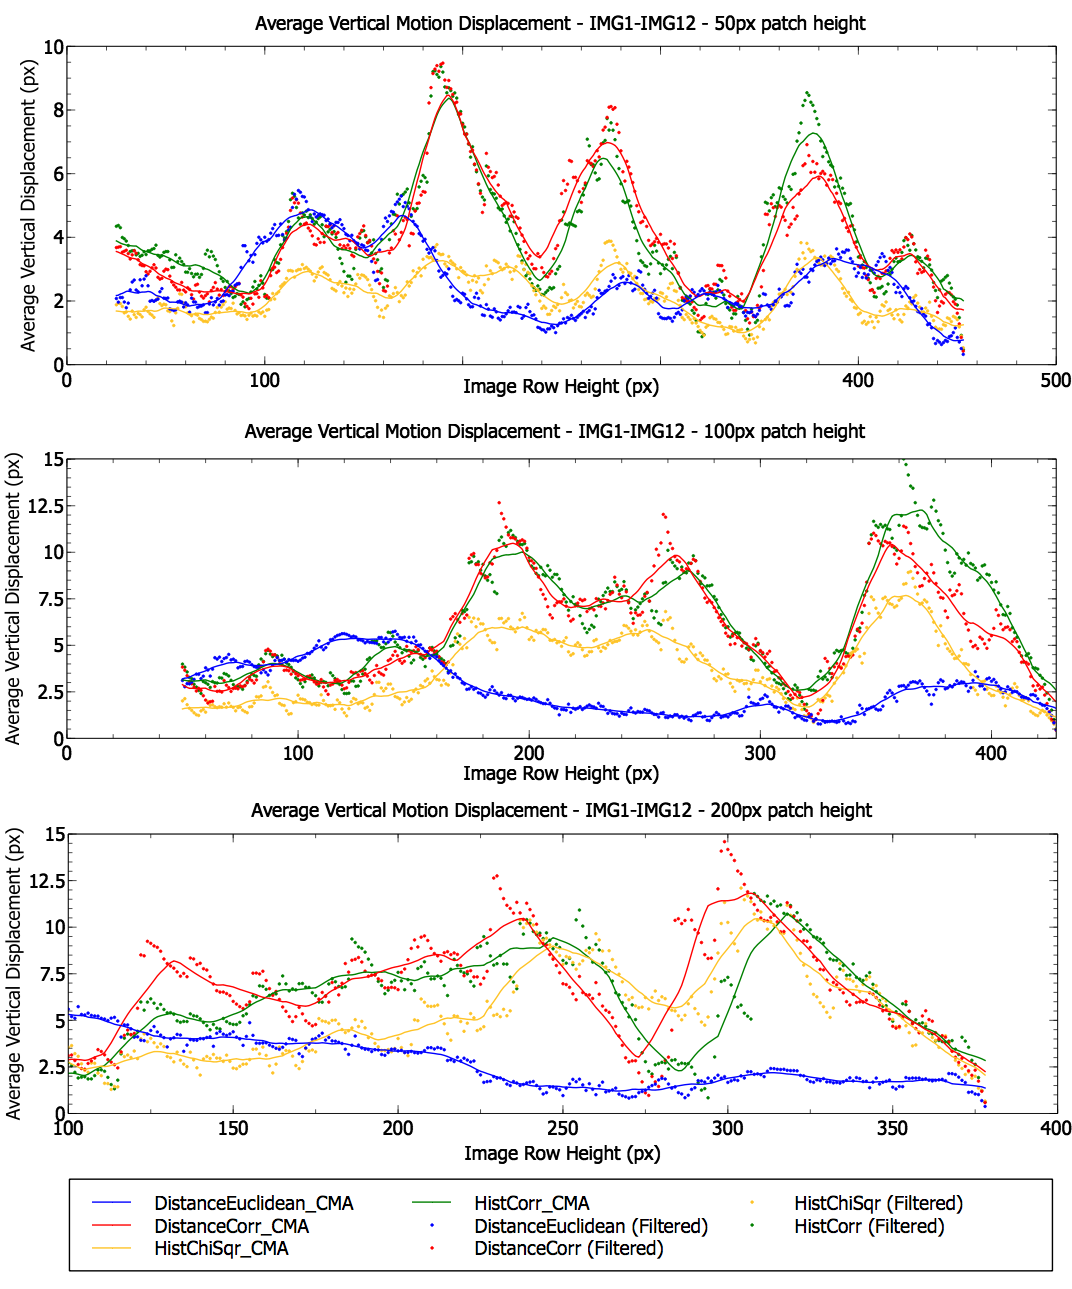
\includegraphics[scale=0.4]{images/results/ex1_results_inside_10cm}
\caption{Average vertical motion displacement models across all images within ``asian rug" dataset running \textit{non-exhaustive} localised search. Graph 1 (Top) - Overlapping patches of 50px-square; Graph 2 (Middle) Overlapping patches of 100px-square; Graph 3 (Bottom) Overlapping patches of 200px-square. Solid line indicates centred moving average (10-pixel interval) calculated from filtered results for each appearance-based template matching similarity metric.}
\label{fig:ex1_1_3}
\end{figure}

Within the results for dataset three (Figure \ref{fig:ex1_1_3}), the vertical displacement shown Graph 1 (50px patch) demonstrates a high level of distortion with no distinct correlation with the vertical height of the row within the image. While the results within Graphs 2 and 3 also demonstrate no particular positive correlation between the row within the image, and the vertical displacement that is demonstrated, they do both appear to identify a sudden decrease in displacement at the same vertical height in the image (approx. 275px for 100px patch and 350px for 200px patch).

\clearpage
\subsubsection{Dataset 4: Slate Footpath (Outdoors)}

\begin{figure}[ht!]
\centering
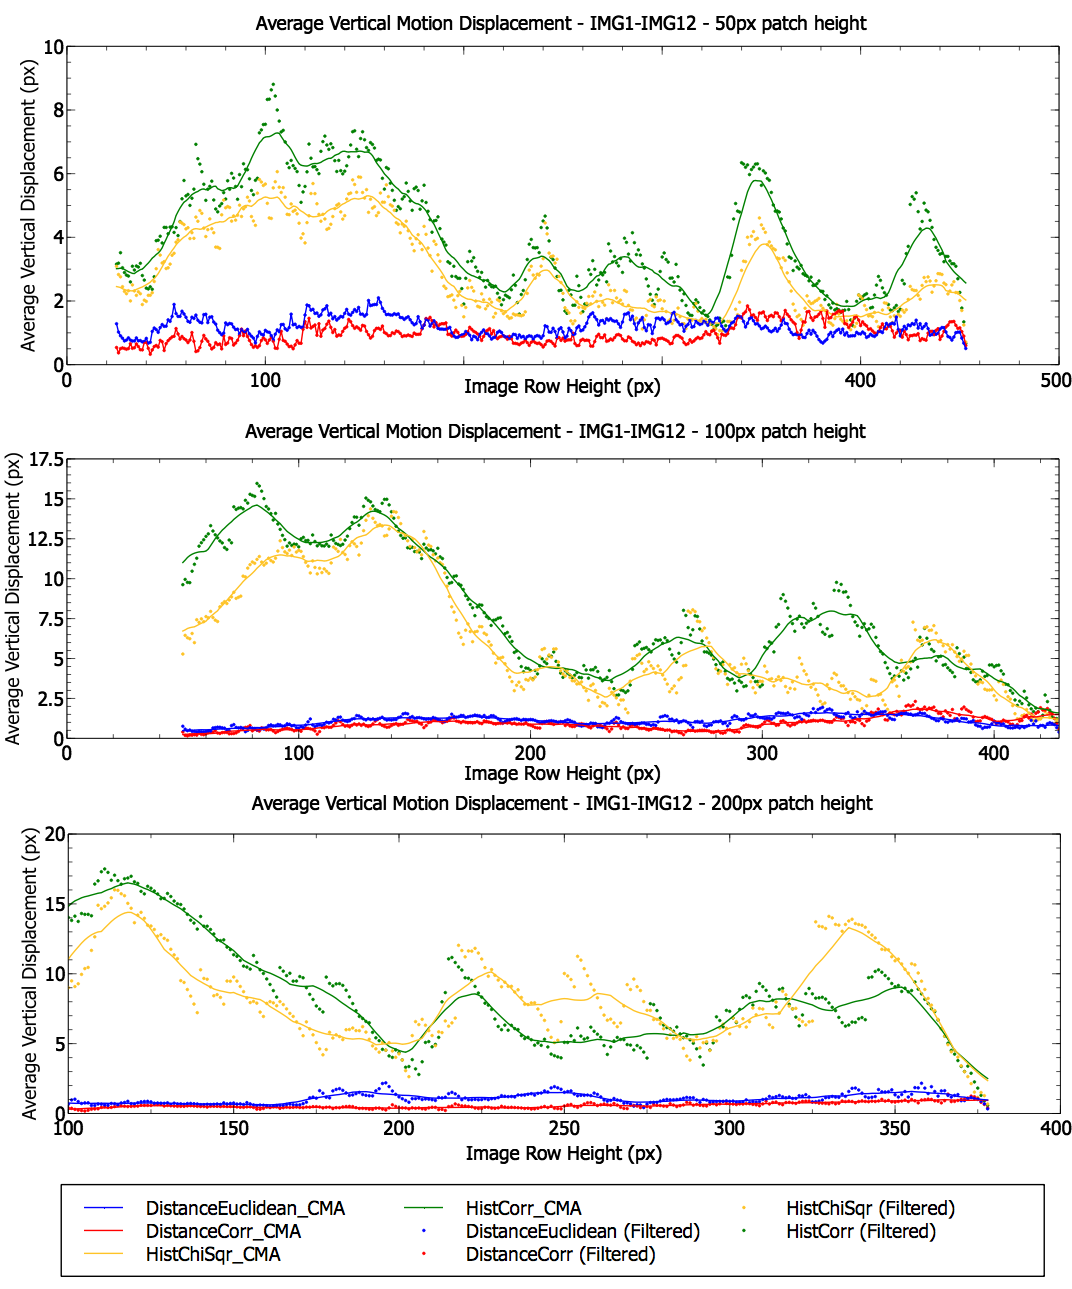
\includegraphics[scale=0.4]{images/results/ex1_results_path_outside_10cm}
\caption{Average vertical motion displacement models across all images within ``slate footpath" dataset running \textit{non-exhaustive} localised search. Graph 1 (Top) - Overlapping patches of 50px-square; Graph 2 (Middle) Overlapping patches of 100px-square; Graph 3 (Bottom) Overlapping patches of 200px-square. Solid line indicates centred moving average (10-pixel interval) calculated from filtered results for each appearance-based template matching similarity metric.}
\label{fig:ex1_1_4}
\end{figure}


The results within Figure \ref{fig:ex1_1_4}, the tests across all three patch sizes appear to indicate similar results, with a clear divide visible between the performance of the histogram-based, and distance-based similarity measures. Of particular interest is the unexpected negative-correlation trend recorded by the histogram-based similarity measures that appears within all three of the graphs, potentially indicate an issue within the dataset.


\clearpage
\subsection{Experiment 2: Template Matching (Full-width Patches - Non-Scaled)}

\subsubsection{Dataset 1: Living Room Carpet (Indoors)}

\begin{figure}[ht!]
\centering
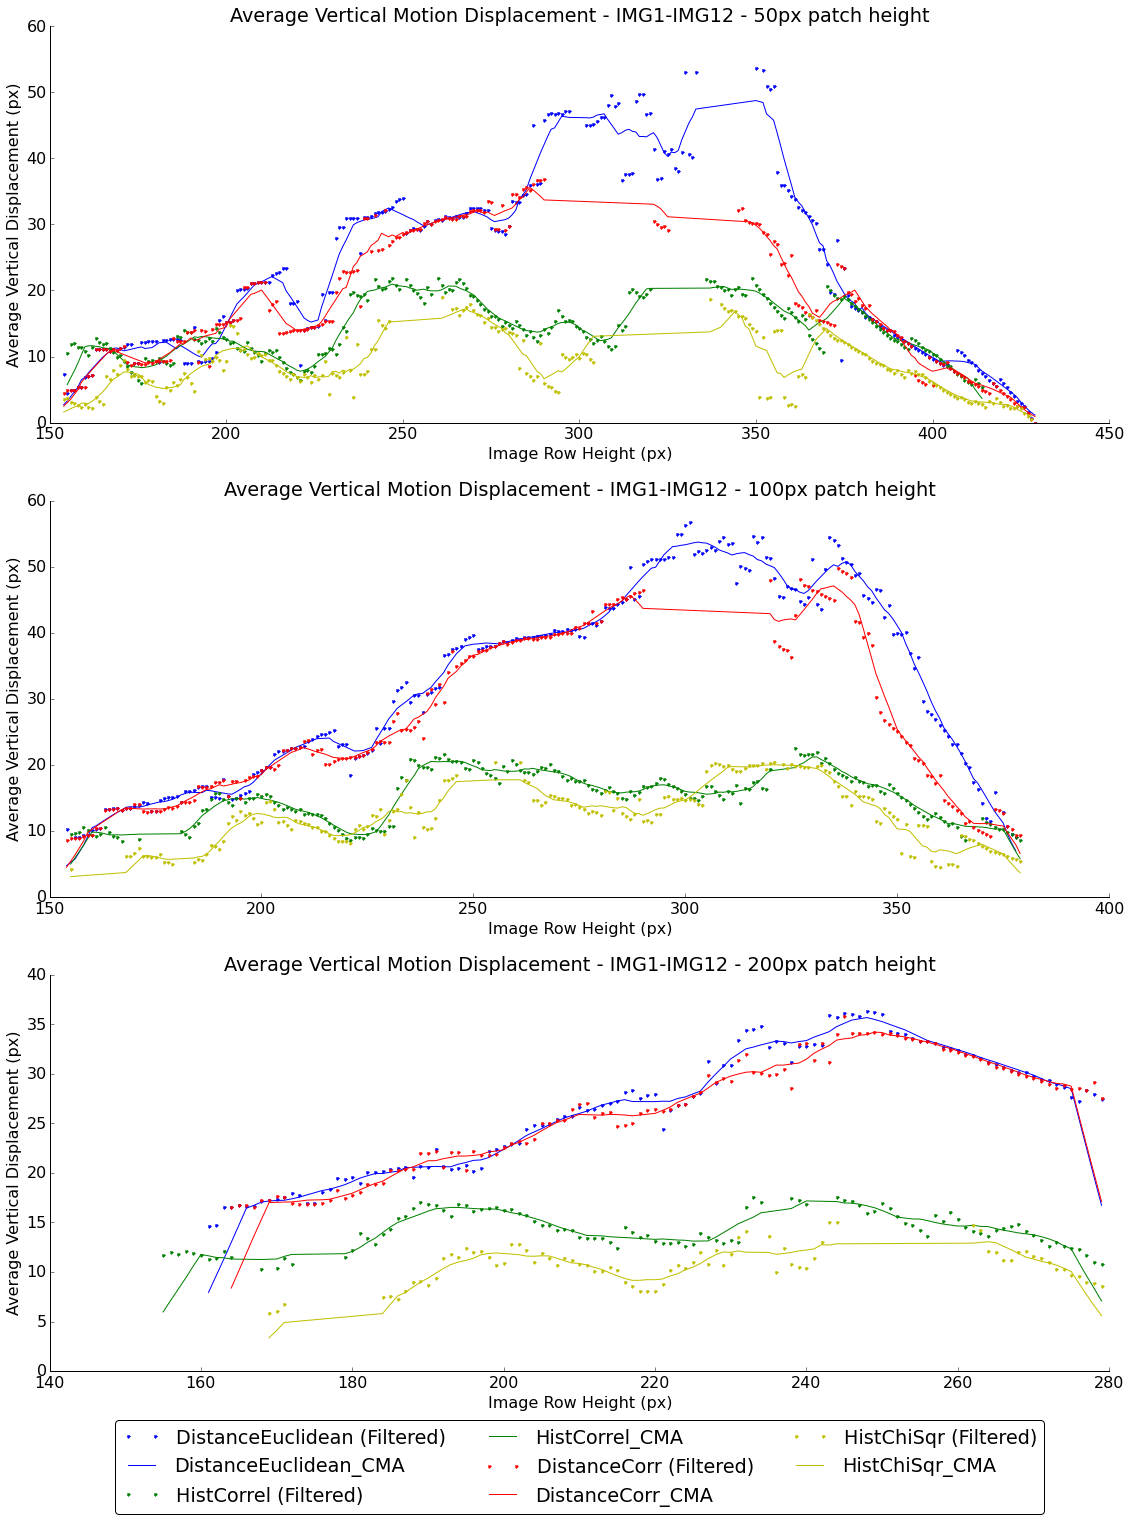
\includegraphics[scale=0.3]{images/results/flat_10cm_non_scaled}
\caption{Average vertical motion displacement models across all images within ``living room carpet" dataset running \textit{non-exhaustive} localised search. Graph 1 (Top) - Full-width patch with fixed height of 50px; Graph 2 (Middle) Full-width patch with fixed height of 100px; Graph 3 (Bottom) Full-width patch with fixed height of 200px. Solid line indicates centred moving average (10-pixel interval) calculated from filtered results for each appearance-based template matching similarity metric.}
\label{fig:ex2_1_1}
\end{figure}

\clearpage
\begin{figure}[ht!]
\centering
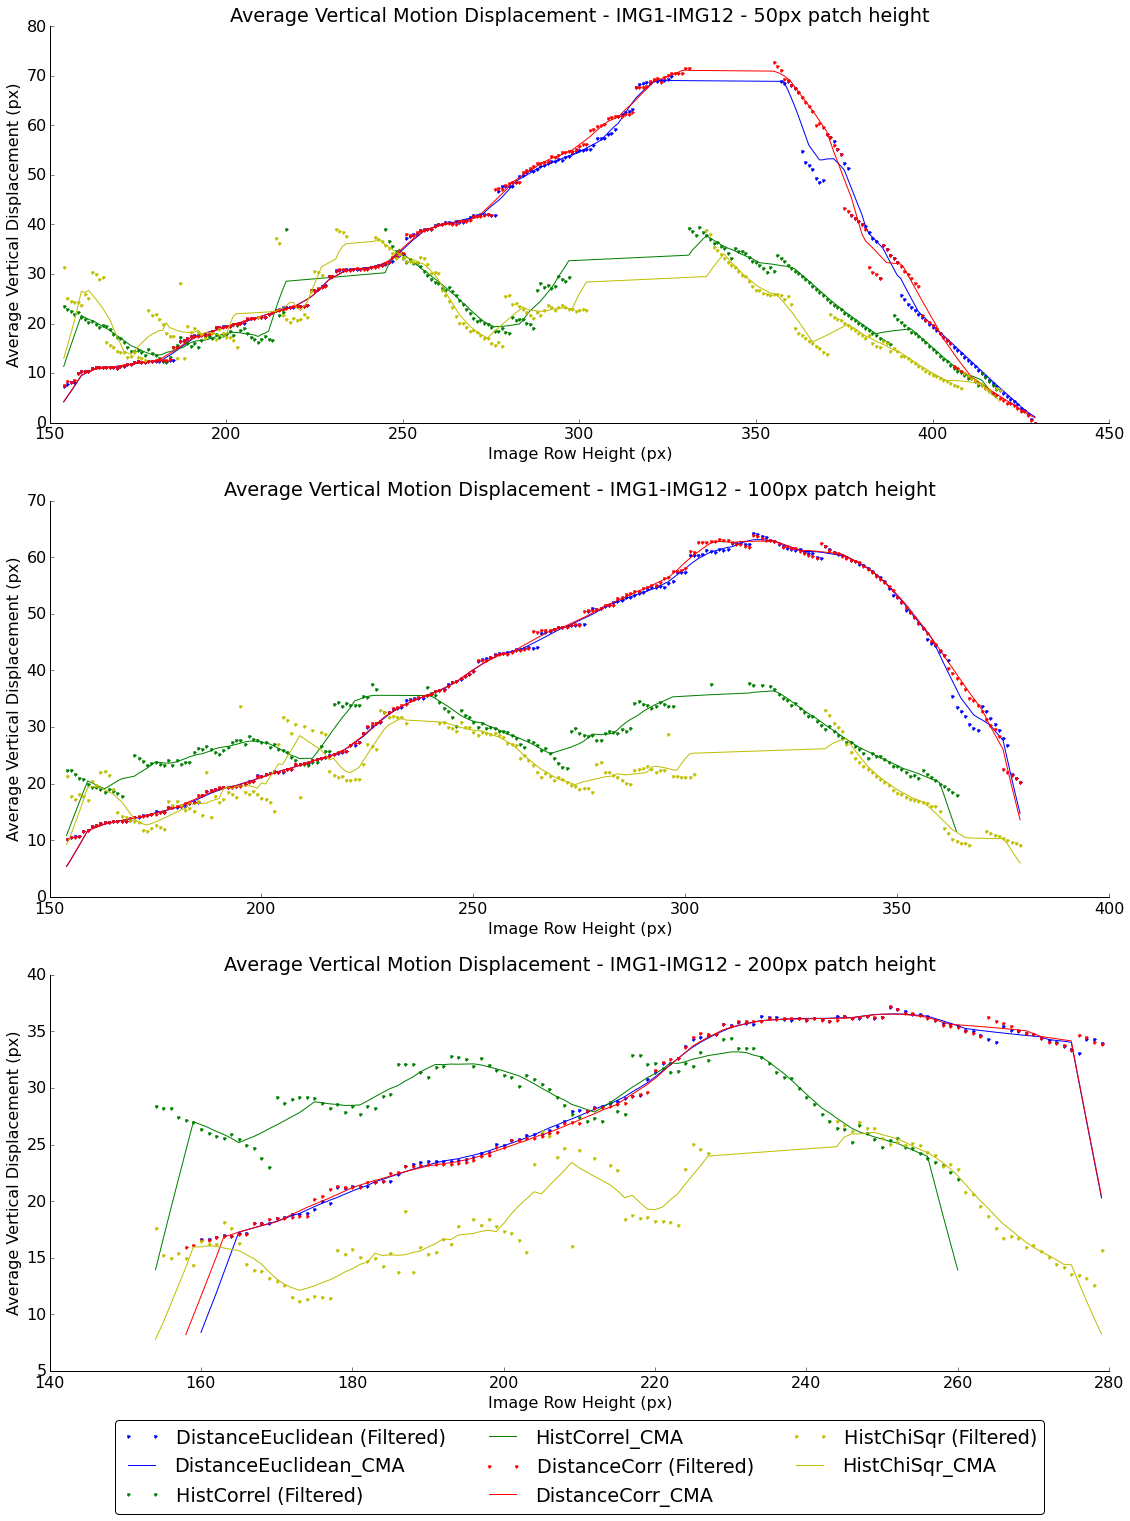
\includegraphics[scale=0.3]{images/results/flat_10cm_non_scaled_exhaustive}
\caption{Average vertical motion displacement models across all images within ``living room carpet" dataset running \textit{exhaustive} localised search. Graph 1 (Top) - Full-width patch with fixed height of 50px; Graph 2 (Middle) Full-width patch with fixed height of 100px; Graph 3 (Bottom) Full-width patch with fixed height of 200px. Solid line indicates centred moving average (10-pixel interval) calculated from filtered results for each appearance-based template matching similarity metric.}
\label{fig:ex2_1_2}
\end{figure}

Across the non-exhaustive, and exhaustive tests for dataset one (Figures \ref{fig:ex2_1_1} and \ref{fig:ex2_1_2} respectively) the two distance-based similarity measures provide clear examples of the expected positive relationship between the row within the image, and the level of vertical displacement. However, in the case of all three of the tested patch sizes, the results from the exhaustive search indicate a significantly smoother upwards trend than the non-exhaustive search.

\clearpage
\subsubsection{Dataset 2: Brick-Paved Road (Outside)}

\begin{figure}[ht!]
\centering
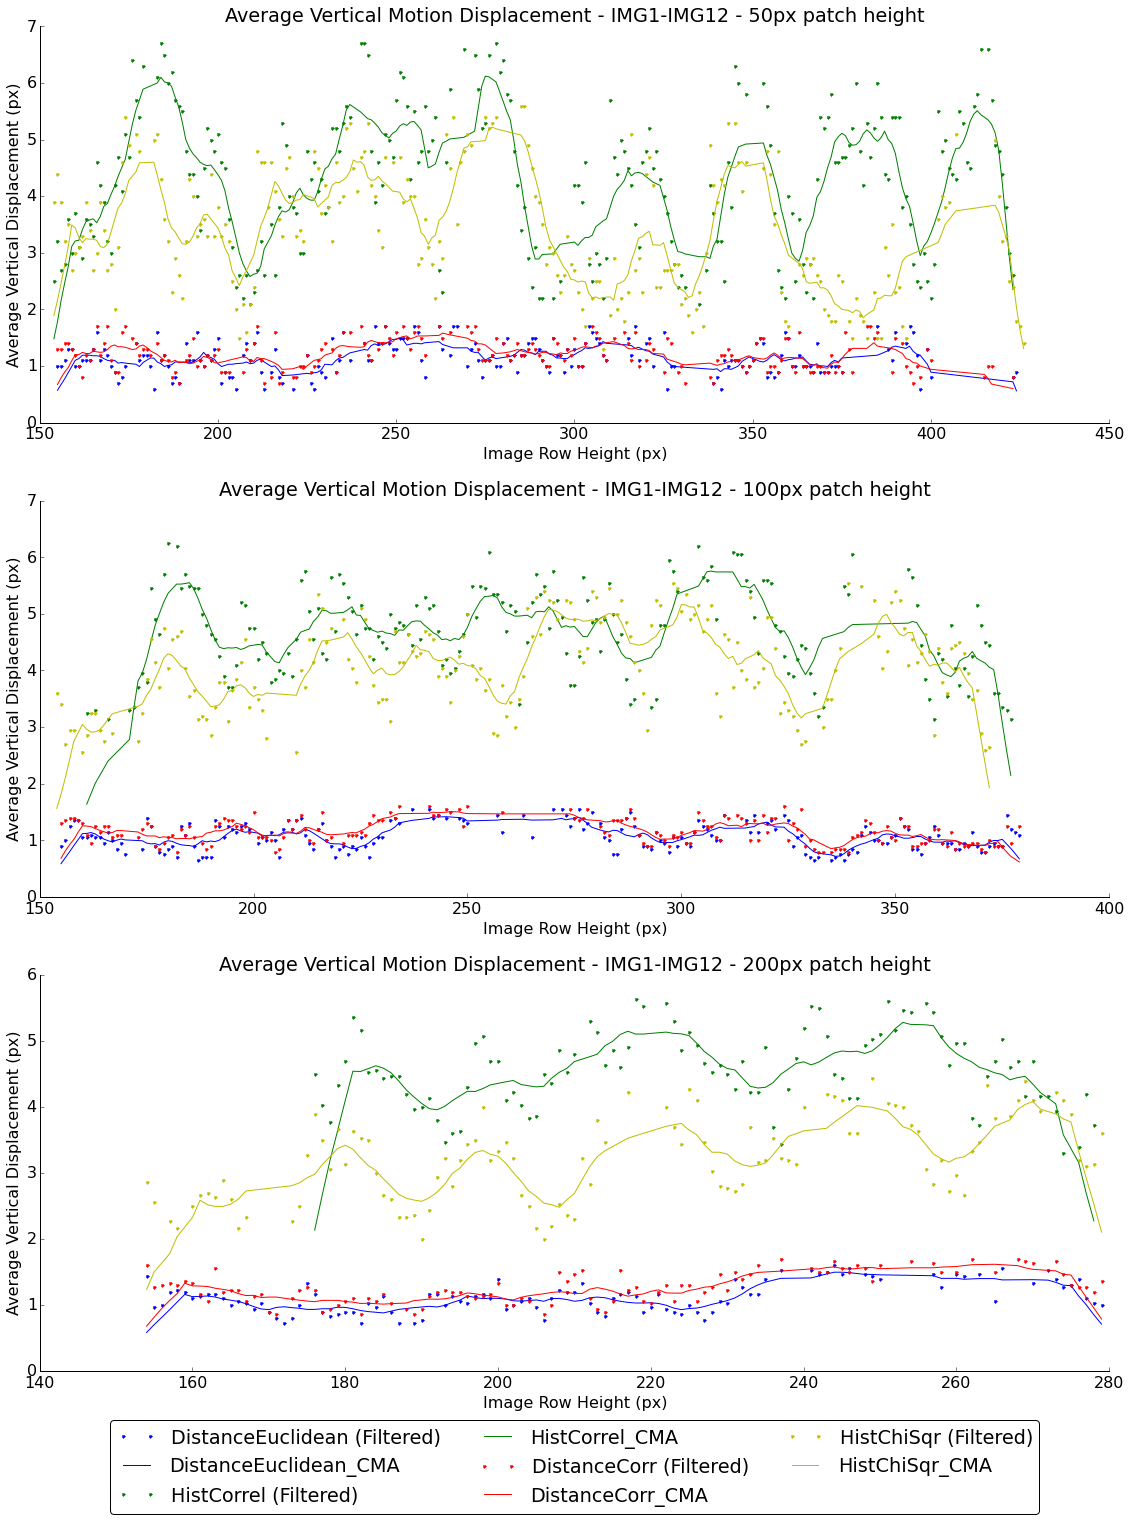
\includegraphics[scale=0.3]{images/results/wiltshire_outside_10cm_non_scaled}
\caption{Average vertical motion displacement models across all images within ``brick-paved drive" dataset running \textit{non-exhaustive} localised search. Graph 1 (Top) - Full-width patch with fixed height of 50px; Graph 2 (Middle) Full-width patch with fixed height of 100px; Graph 3 (Bottom) Full-width patch with fixed height of 200px. Solid line indicates centred moving average (10-pixel interval) calculated from filtered results for each appearance-based template matching similarity metric.}
\label{fig:ex2_2_1}
\end{figure}

\clearpage
\begin{figure}[ht!]
\centering
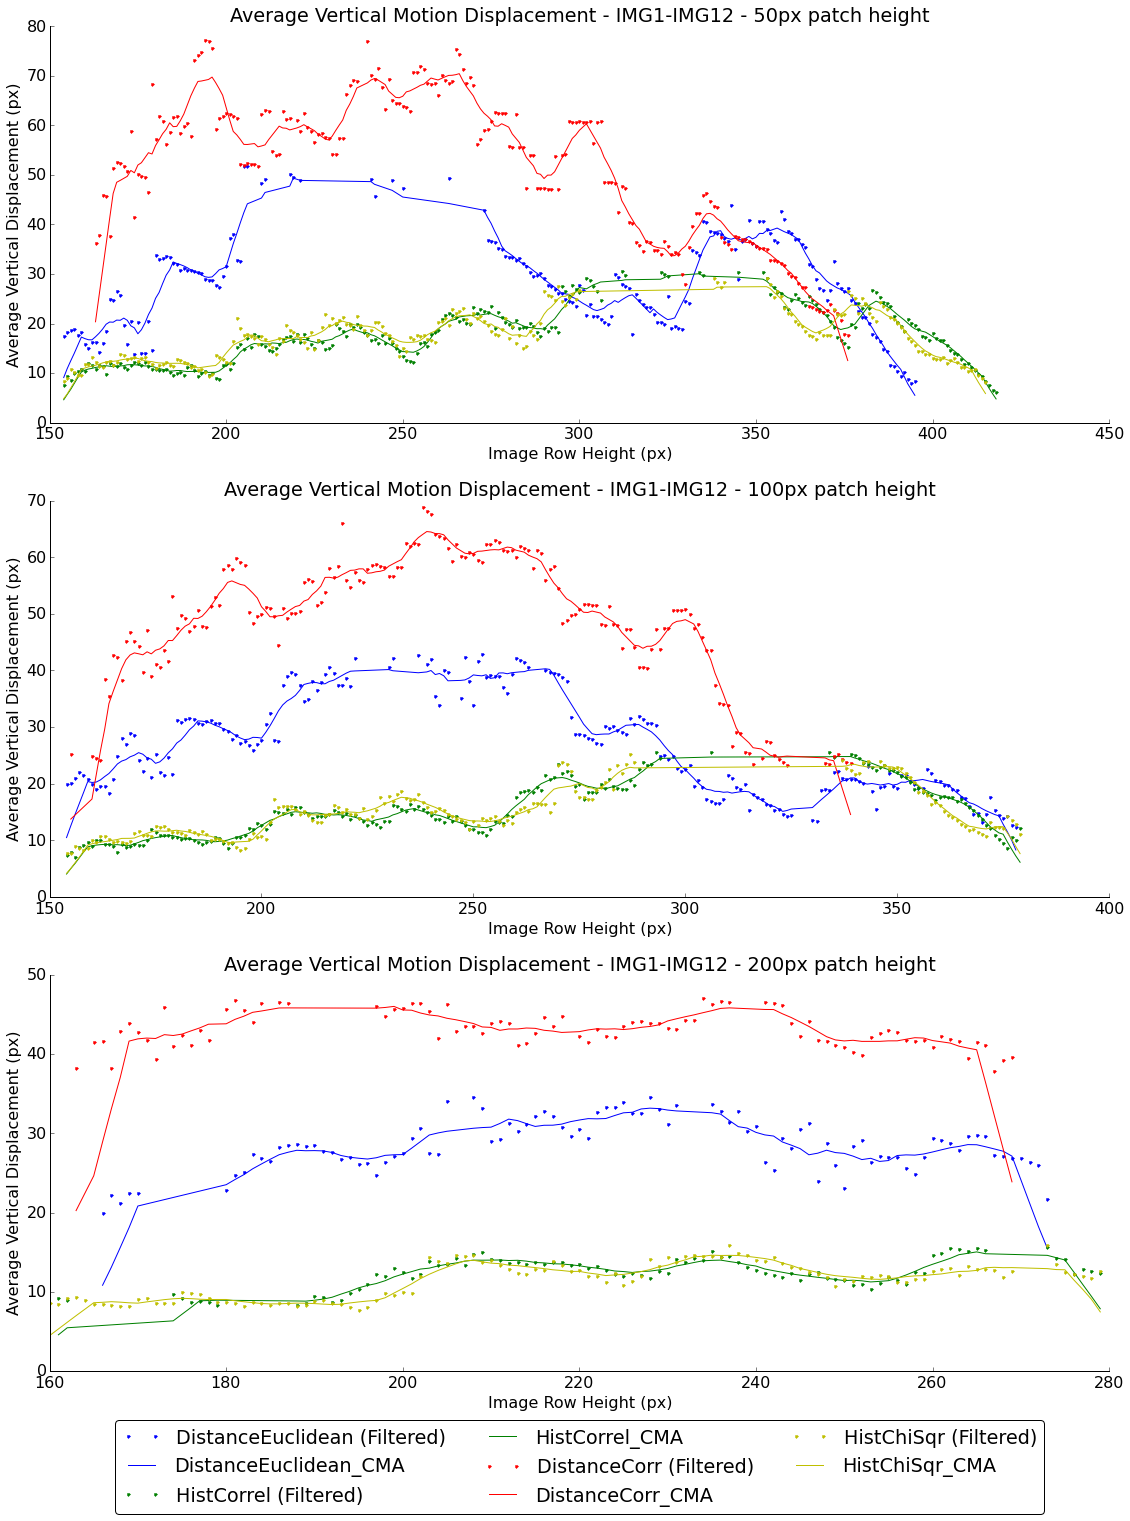
\includegraphics[scale=0.3]{images/results/wiltshire_outside_10cm_non_scaled_exhaustive}
\caption{Average vertical motion displacement models across all images within ``brick-paved drive" dataset running \textit{exhaustive} localised search. Graph 1 (Top) - Full-width patch with fixed height of 50px; Graph 2 (Middle) Full-width patch with fixed height of 100px; Graph 3 (Bottom) Full-width patch with fixed height of 200px. Solid line indicates centred moving average (10-pixel interval) calculated from filtered results for each appearance-based template matching similarity metric.}
\label{fig:ex2_2_2}
\end{figure}

The results recorded between the non-exhaustive, and exhaustive tests for dataset two (Figures \ref{fig:ex2_2_1} and \ref{fig:ex2_2_2} respectively) provide a stark contrast in performance between the two categories of similarity measure. Within the results of the non-exhaustive search, the two histogram-based measures indicate proportionally greater levels of displacement than the Normalised Cross-Correlation and Euclidean Distance measures. However this recorded displacement also demonstrates a considerable level of noise. In contrast, the results for the exhaustive search show greater levels of vertical displacement overall, but in this case it is the Euclidean Distance that provides the highest displacement, with Normalised Cross Correlation coming second.  

\clearpage
\subsubsection{Dataset 3: Asian Rug (Indoors)}

\begin{figure}[ht!]
\centering
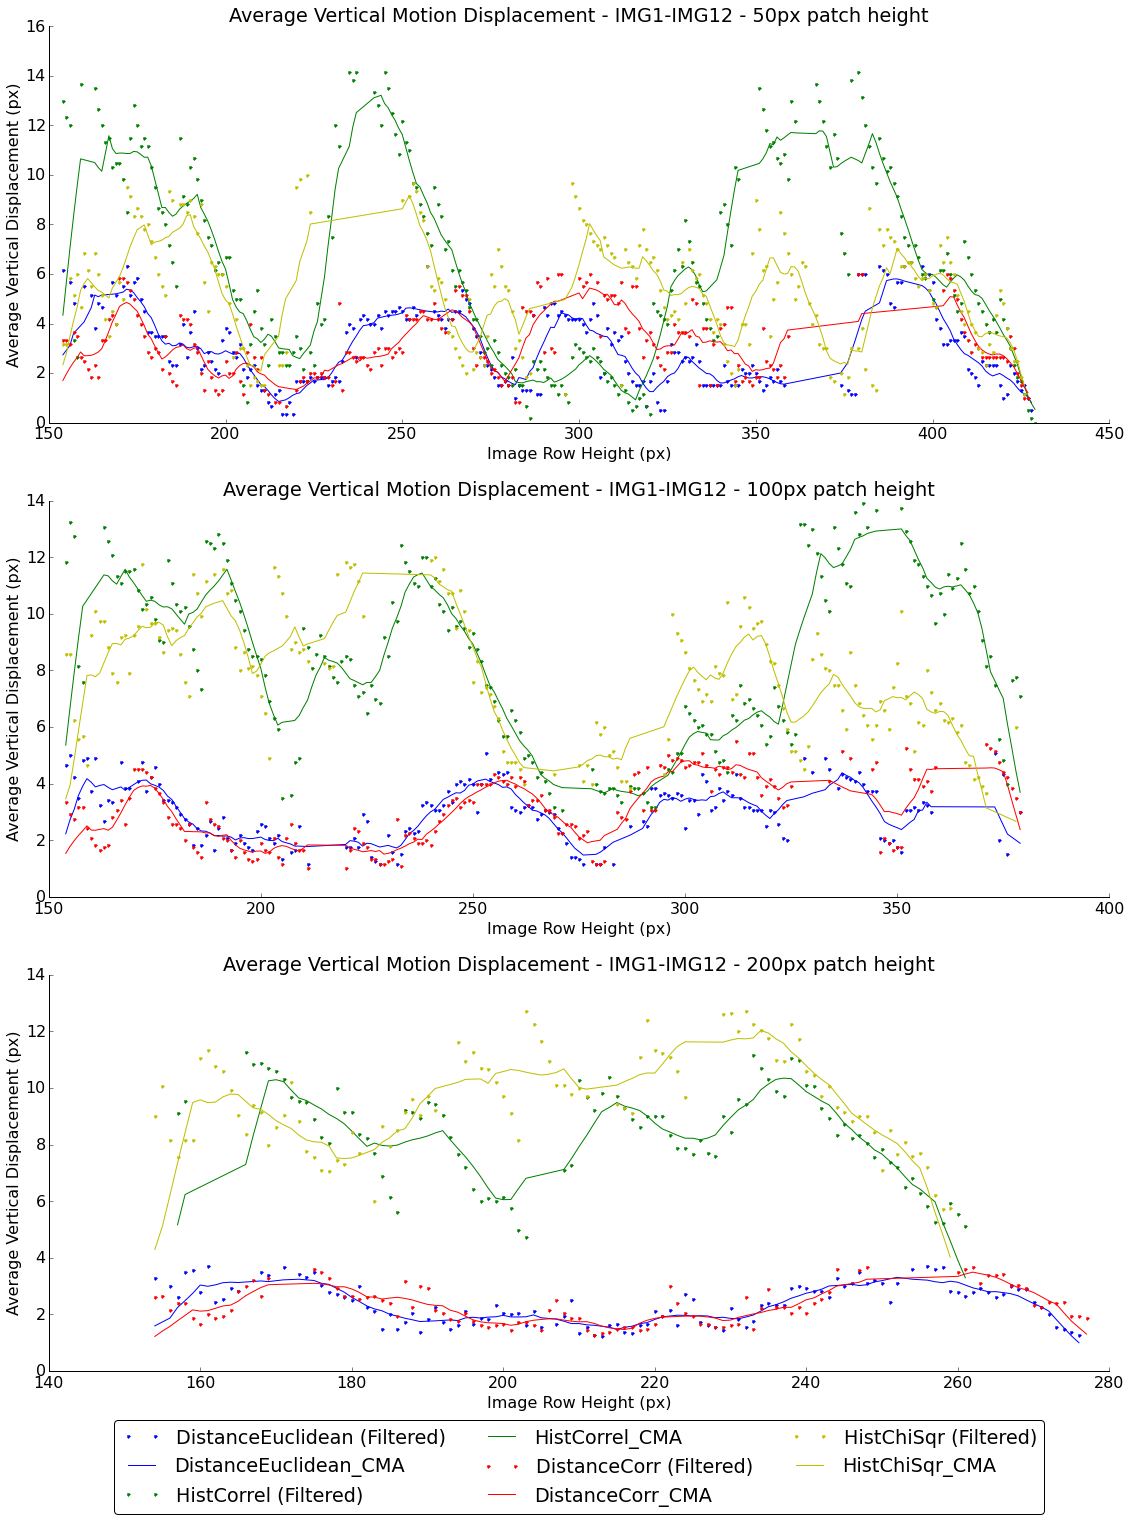
\includegraphics[scale=0.3]{images/results/wiltshire_inside_10cm_non_scaled}
\caption{Average vertical motion displacement models across all images within ``asian rug" dataset running \textit{non-exhaustive} localised search. Graph 1 (Top) - Full-width patch with fixed height of 50px; Graph 2 (Middle) Full-width patch with fixed height of 100px; Graph 3 (Bottom) Full-width patch with fixed height of 200px. Solid line indicates centred moving average (10-pixel interval) calculated from filtered results for each appearance-based template matching similarity metric.}
\label{fig:ex2_3_1}
\end{figure}

\clearpage
\begin{figure}[ht!]
\centering
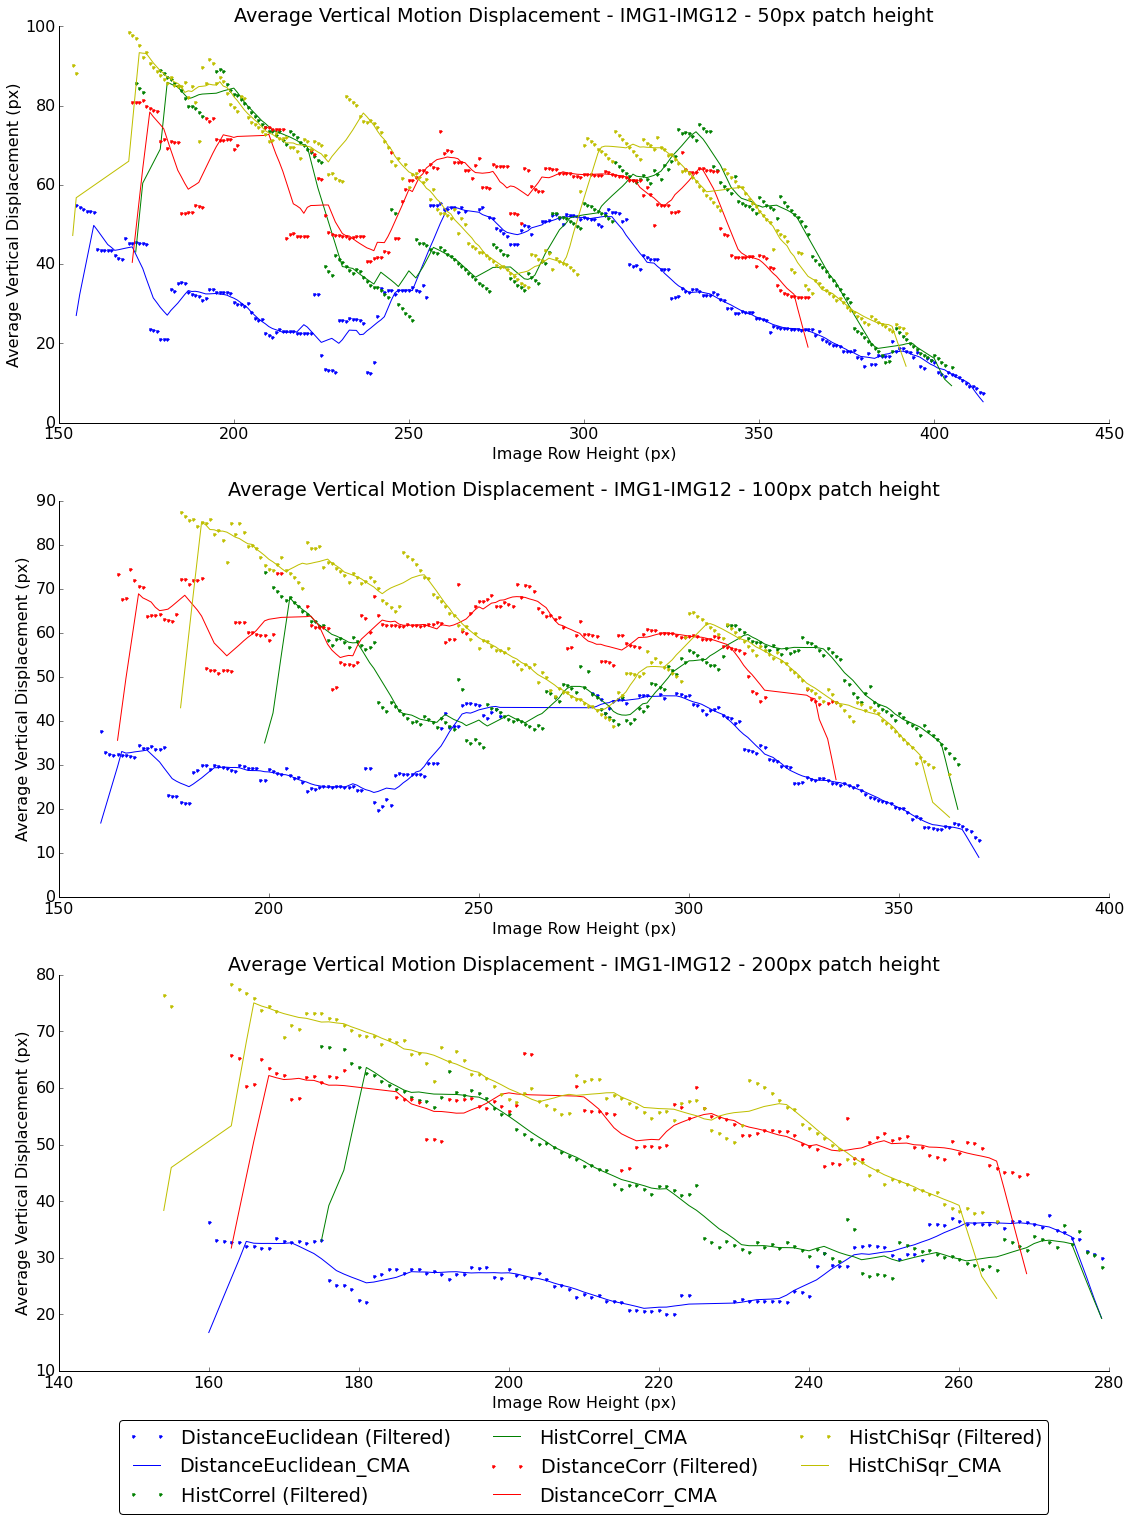
\includegraphics[scale=0.3]{images/results/wiltshire_inside_10cm_non_scaled_exhaustive}
\caption{Average vertical motion displacement models across all images within ``asian rug" dataset running \textit{exhaustive} localised search. Graph 1 (Top) - Full-width patch with fixed height of 50px; Graph 2 (Middle) Full-width patch with fixed height of 100px; Graph 3 (Bottom) Full-width patch with fixed height of 200px. Solid line indicates centred moving average (10-pixel interval) calculated from filtered results for each appearance-based template matching similarity metric.}
\label{fig:ex2_3_2}
\end{figure}

For dataset three, neither the exhaustive (Figure \ref{fig:ex2_3_1}), or non-exhaustive (Figure \ref{fig:ex2_3_2}) localised search approaches provide particularly desirable results, with all of the patch sizes and similarity measures demonstrating either just significant levels of noise with no correlation between image row and vertical displacement demonstrated, or in the case of the exhaustive search, less overall noise but a negative correlation, hence showing the opposite trend of what is expected. 

\clearpage
\subsubsection{Dataset 4: Slate Footpath (Outdoors)}

\begin{figure}[ht!]
\centering
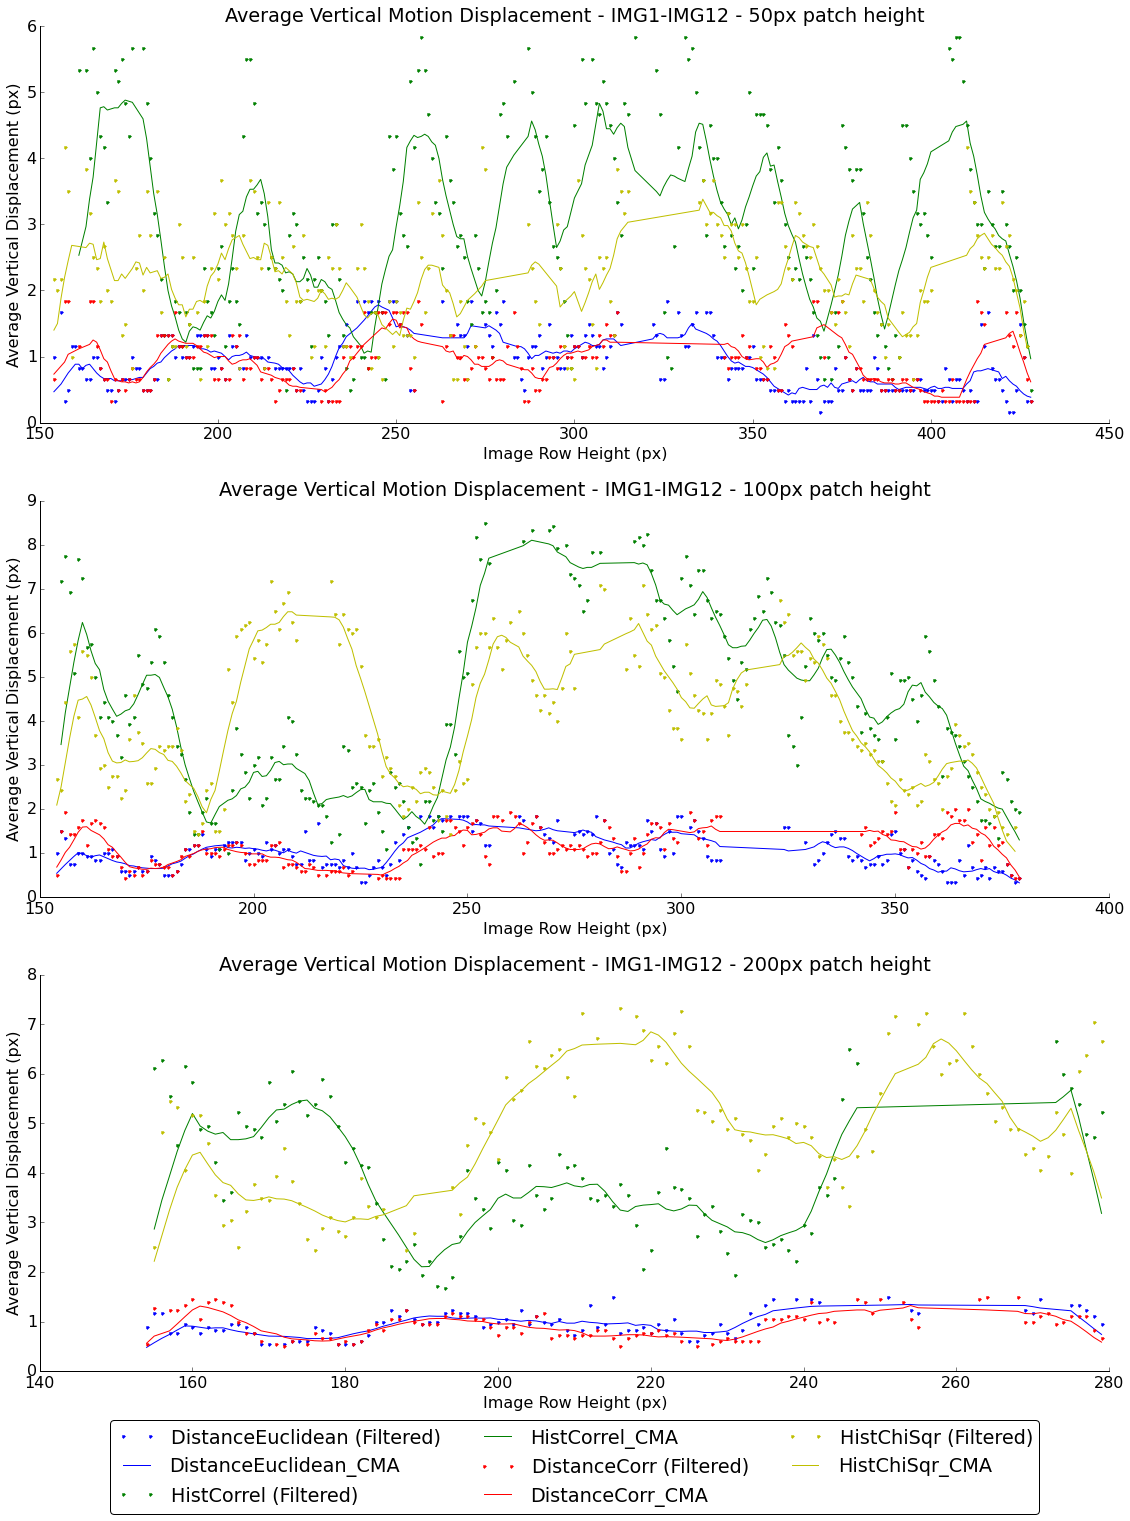
\includegraphics[scale=0.3]{images/results/path_outside_10cm_non_scaled}
\caption{Average vertical motion displacement models across all images within ``slate footpath" dataset running \textit{non-exhaustive} localised search. Graph 1 (Top) - Full-width patch with fixed height of 50px; Graph 2 (Middle) Full-width patch with fixed height of 100px; Graph 3 (Bottom) Full-width patch with fixed height of 200px. Solid line indicates centred moving average (10-pixel interval) calculated from filtered results for each appearance-based template matching similarity metric.}
\label{fig:ex2_4_1}
\end{figure}

\clearpage
\begin{figure}[ht!]
\centering
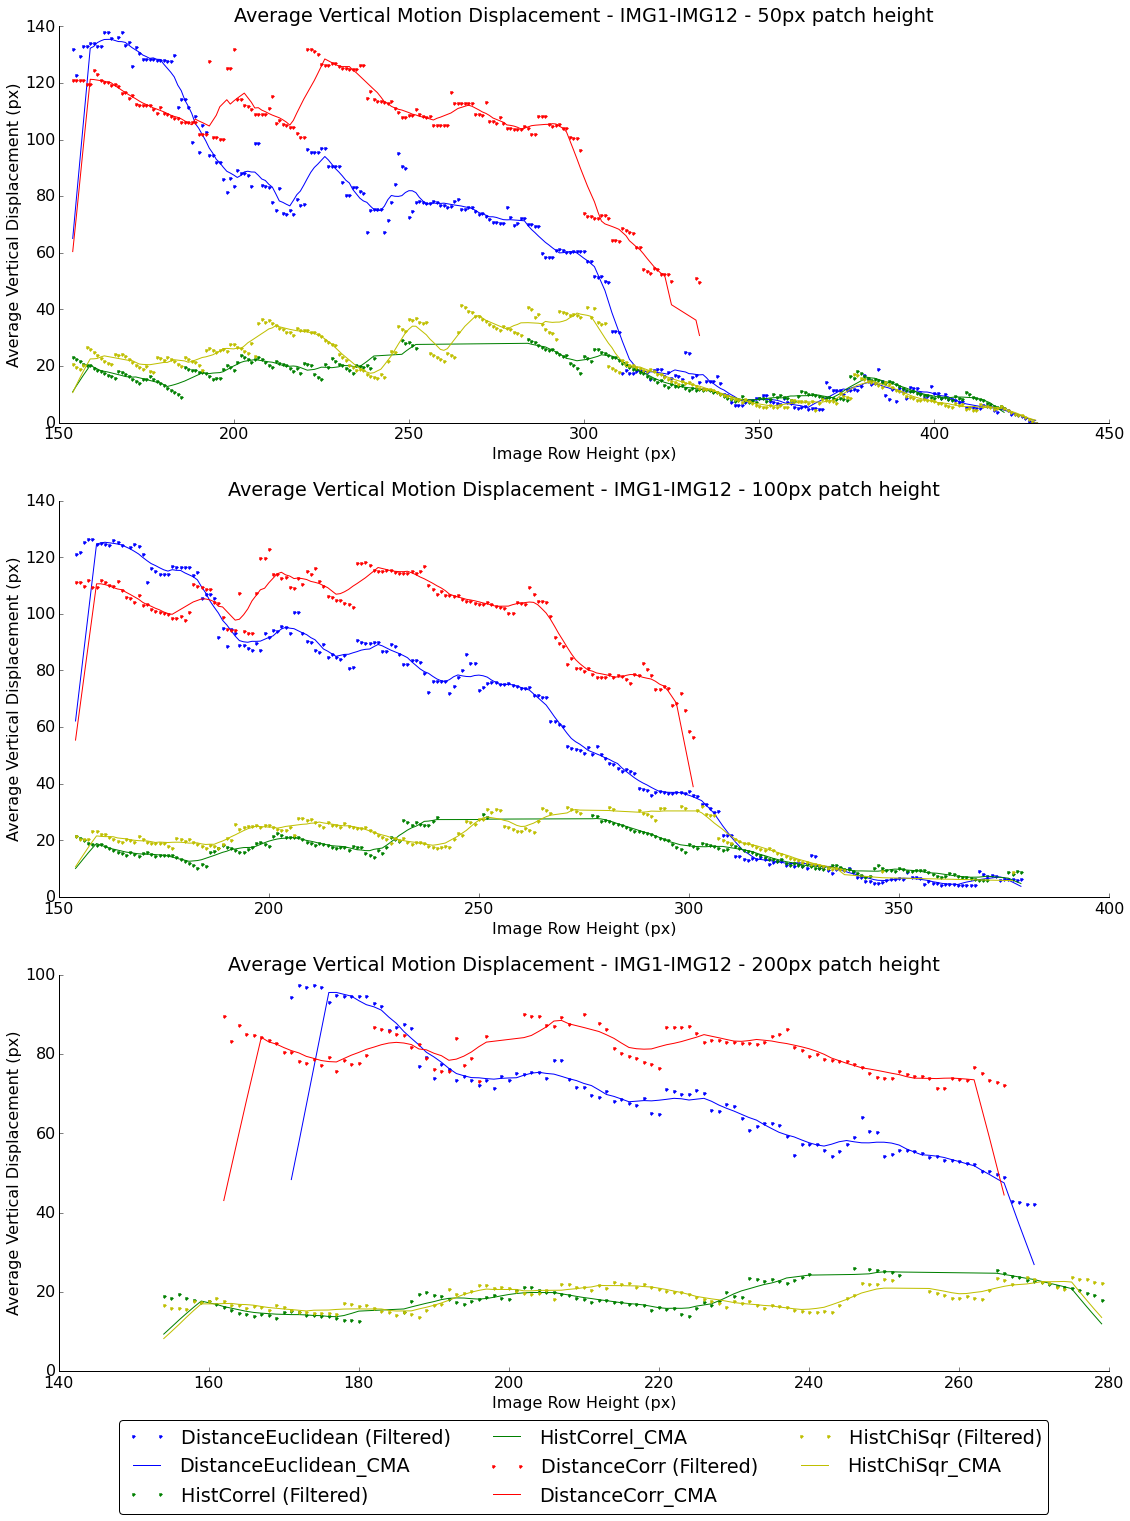
\includegraphics[scale=0.3]{images/results/path_outside_10cm_non_scaled_exhaustive}
\caption{Average vertical motion displacement models across all images within ``slate footpath" dataset running \textit{exhaustive} localised search. Graph 1 (Top) - Full-width patch with fixed height of 50px; Graph 2 (Middle) Full-width patch with fixed height of 100px; Graph 3 (Bottom) Full-width patch with fixed height of 200px. Solid line indicates centred moving average (10-pixel interval) calculated from filtered results for each appearance-based template matching similarity metric.}
\label{fig:ex2_4_2}
\end{figure}


The results for dataset four (Figures \ref{fig:ex2_4_1} and \ref{fig:ex2_4_2}) resemble those shown for the previous dataset (Figures \ref{fig:ex2_3_1} and \ref{fig:ex2_3_2}) whereby the non-exhaustive search results indicate high levels of noise and for exhaustive search results, while all patch sizes do indicate a definitive correlation between row height and the demonstrated vertical displacement, it is again a negative, rather than expected positive correlation. 

\clearpage
\subsection{Experiment 3: Template Matching (Full-width Patches - Scaled)}

\subsubsection{Dataset 1: Living Room Carpet (Indoors)}

\begin{figure}[ht!]
\centering
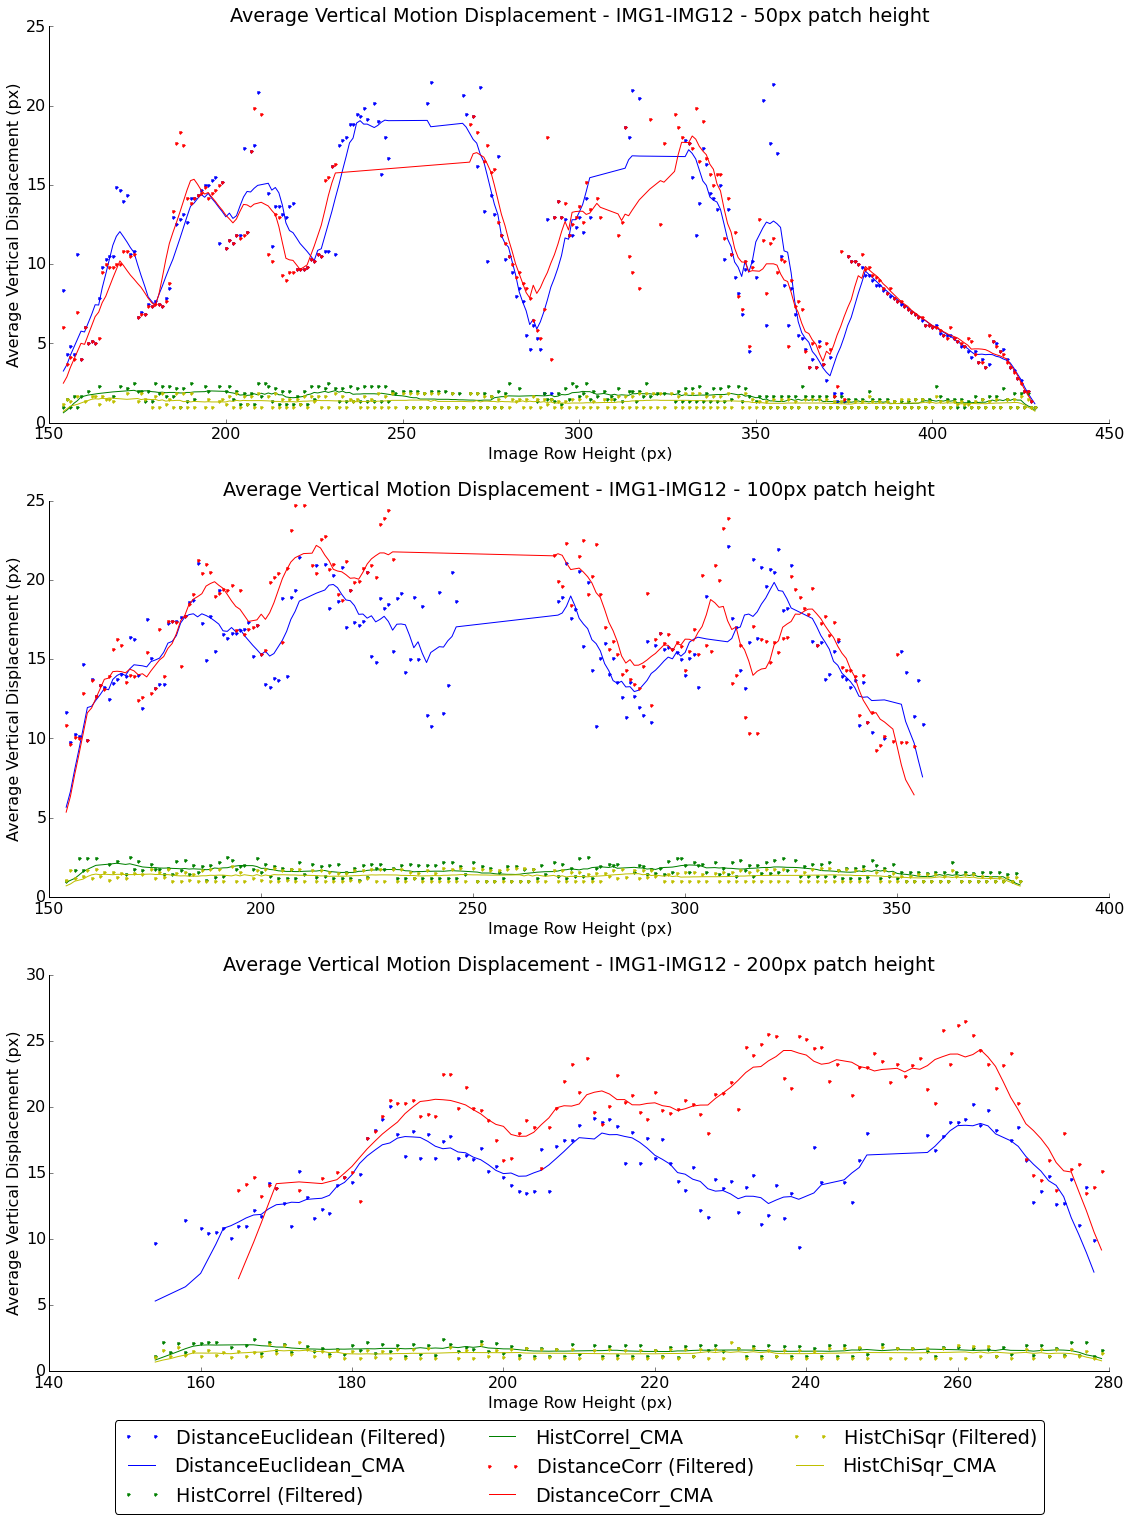
\includegraphics[scale=0.3]{images/results/flat_10cm_scaled}
\caption{Average vertical motion displacement models across all images within ``living room carpet" dataset running \textit{non-exhaustive} localised search with geometrically scaled template patches. Graph 1 (Top) - Full-width patch with fixed height of 50px; Graph 2 (Middle) Full-width patch with fixed height of 100px; Graph 3 (Bottom) Full-width patch with fixed height of 200px. Solid line indicates centred moving average (10-pixel interval) calculated from filtered results for each appearance-based template matching similarity metric.}
\label{fig:ex3_1_1}
\end{figure}

\clearpage
\begin{figure}[ht!]
\centering
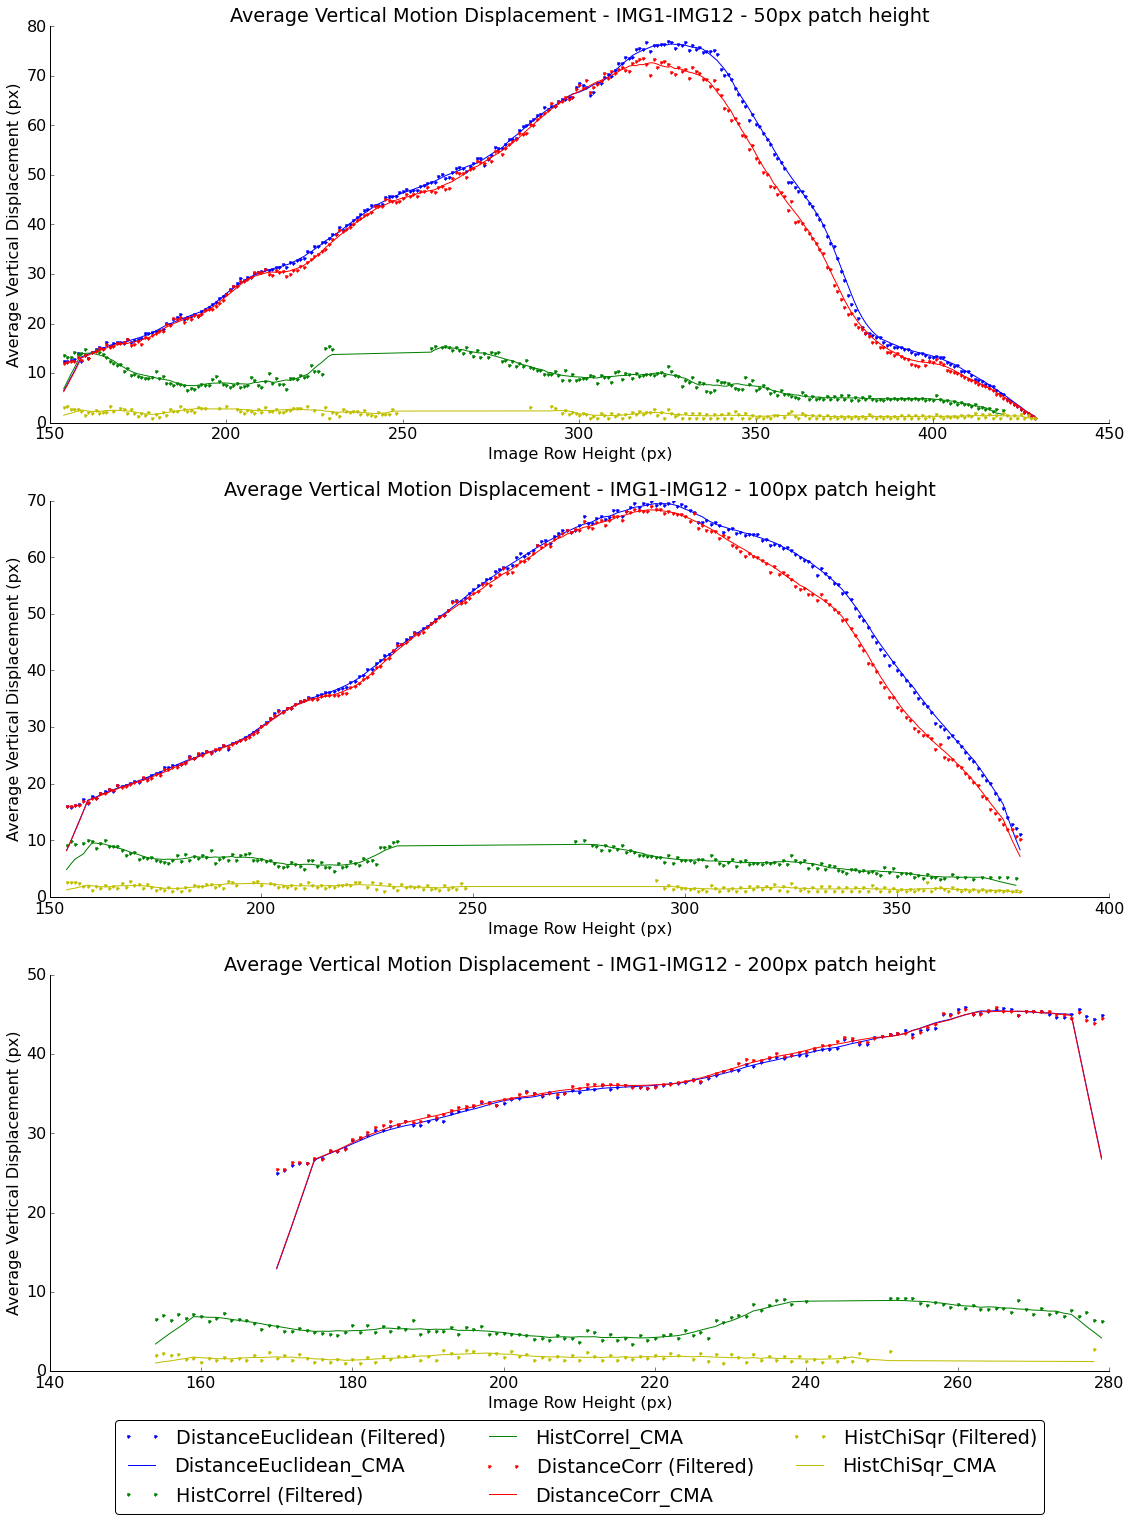
\includegraphics[scale=0.3]{images/results/flat_10cm_scaled_exhaustive}
\caption{Average vertical motion displacement models across all images within ``living room carpet" dataset running \textit{exhaustive} localised search with geometrically scaled template patches. Graph 1 (Top) - Full-width patch with fixed height of 50px; Graph 2 (Middle) Full-width patch with fixed height of 100px; Graph 3 (Bottom) Full-width patch with fixed height of 200px. Solid line indicates centred moving average (10-pixel interval) calculated from filtered results for each appearance-based template matching similarity metric.}
\label{fig:ex3_1_2}
\end{figure}

The results for dataset one appear to indicate a difference between the performance of the non-exhaustive search (Figure \ref{fig:ex3_1_1}) vs the exhaustive search (Figure \ref{fig:ex3_1_2}) when performing scaling of the template patch. Within the non-exhaustive results, while the third test using the 200px-height patch (Fig: \ref{fig:ex3_1_1} Graph 3) does appear to show the expected positive correlation, the tests involving the smaller patches are more susceptible to noise (with the smallest patch showing the most distortion). In contrast to this, all three of the exhaustive searches demonstrate a strong and well defined positive correlation for both of the distance-based similarity measures. For all tests performed on dataset one,the histogram-based approaches to record any significant displacement fails.

\clearpage
\subsubsection{Dataset 2: Brick-Paved Road (Outside)}

\begin{figure}[ht!]
\centering
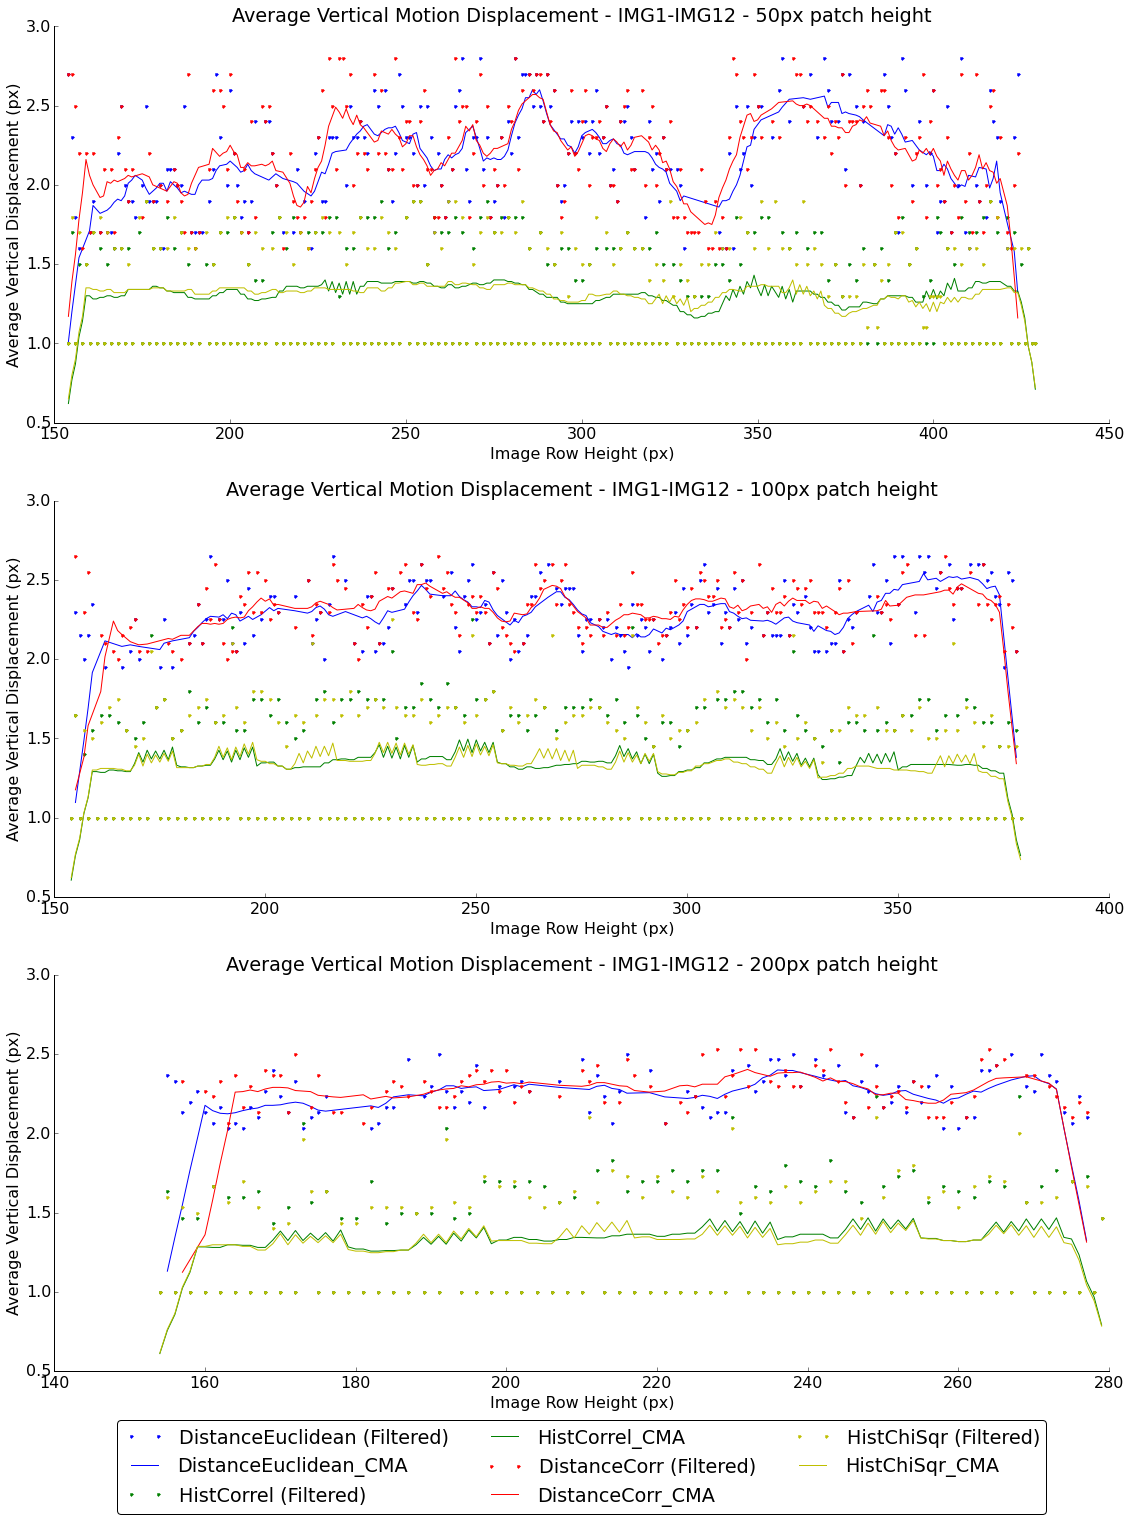
\includegraphics[scale=0.3]{images/results/wiltshire_outside_10cm_scaled}
\caption{Average vertical motion displacement models across all images within ``brick-paved drive" dataset running \textit{non-exhaustive} localised search with geometrically scaled template patches. Graph 1 (Top) - Full-width patch with fixed height of 50px; Graph 2 (Middle) Full-width patch with fixed height of 100px; Graph 3 (Bottom) Full-width patch with fixed height of 200px. Solid line indicates centred moving average (10-pixel interval) calculated from filtered results for each appearance-based template matching similarity metric.}
\label{fig:ex3_2_1}
\end{figure}

\clearpage
\begin{figure}[ht!]
\centering
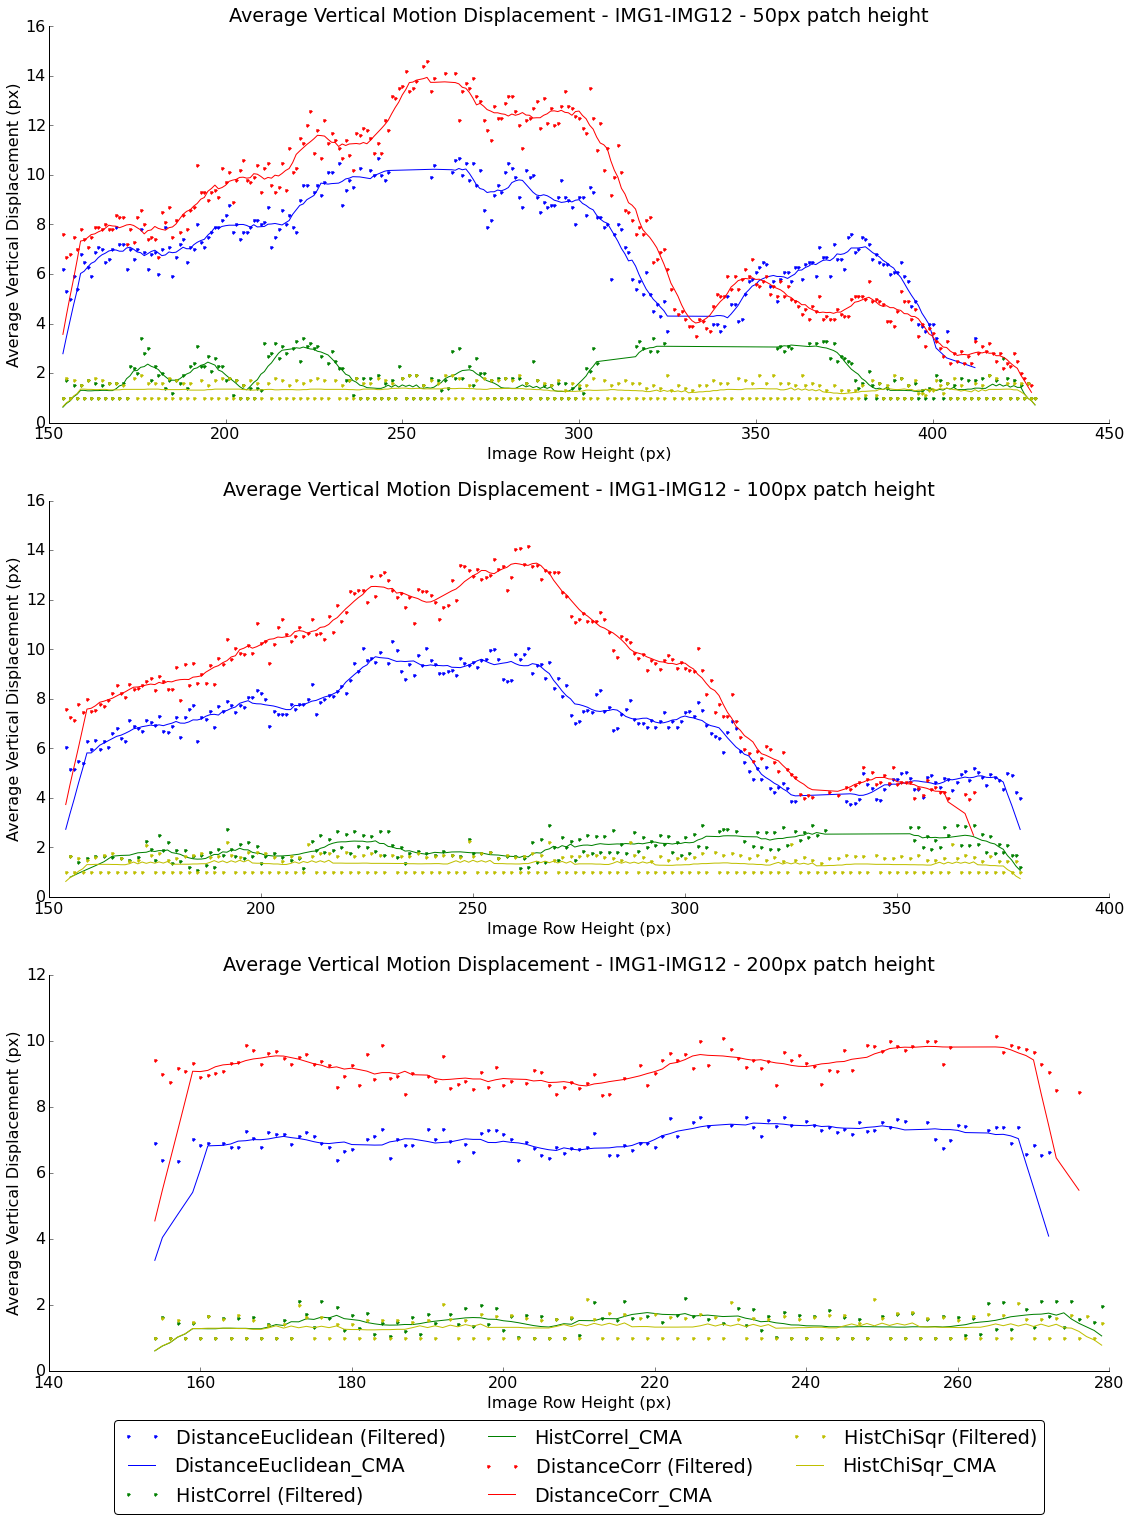
\includegraphics[scale=0.3]{images/results/wiltshire_outside_10cm_scaled_exhaustive}
\caption{Average vertical motion displacement models across all images within ``brick-paved drive" dataset running \textit{exhaustive} localised search with geometrically scaled template patches. Graph 1 (Top) - Full-width patch with fixed height of 50px; Graph 2 (Middle) Full-width patch with fixed height of 100px; Graph 3 (Bottom) Full-width patch with fixed height of 200px. Solid line indicates centred moving average (10-pixel interval) calculated from filtered results for each appearance-based template matching similarity metric.}
\label{fig:ex3_2_2}
\end{figure}

Under the non-exhaustive tests for dataset two (Figure \ref{fig:ex3_2_1}), all four similarity measures appear to indicate an approximately equal level of vertical displacement regardless of the row height, with a small maximum displacement measured (approx. 2-3px). Interestingly, this similar behaviour between the four similarity metrics is demonstrated across all three patches (although the level of noise demonstrated does decrease as the patch size increases). For the exhaustive search (Figure \ref{fig:ex3_2_2}), a general positive correlation does begin to emerge for 50px and 100px patch heights under the distance-based similarity measures, however the results for the 200px patch size appear to show a lack of correlation, in the same way as for the corresponding test within the non-exhaustive results (Fig \ref{fig:ex3_2_1} Chart 3). 

\clearpage
\subsubsection{Dataset 3: Asian Rug (Indoors)}

\begin{figure}[ht!]
\centering
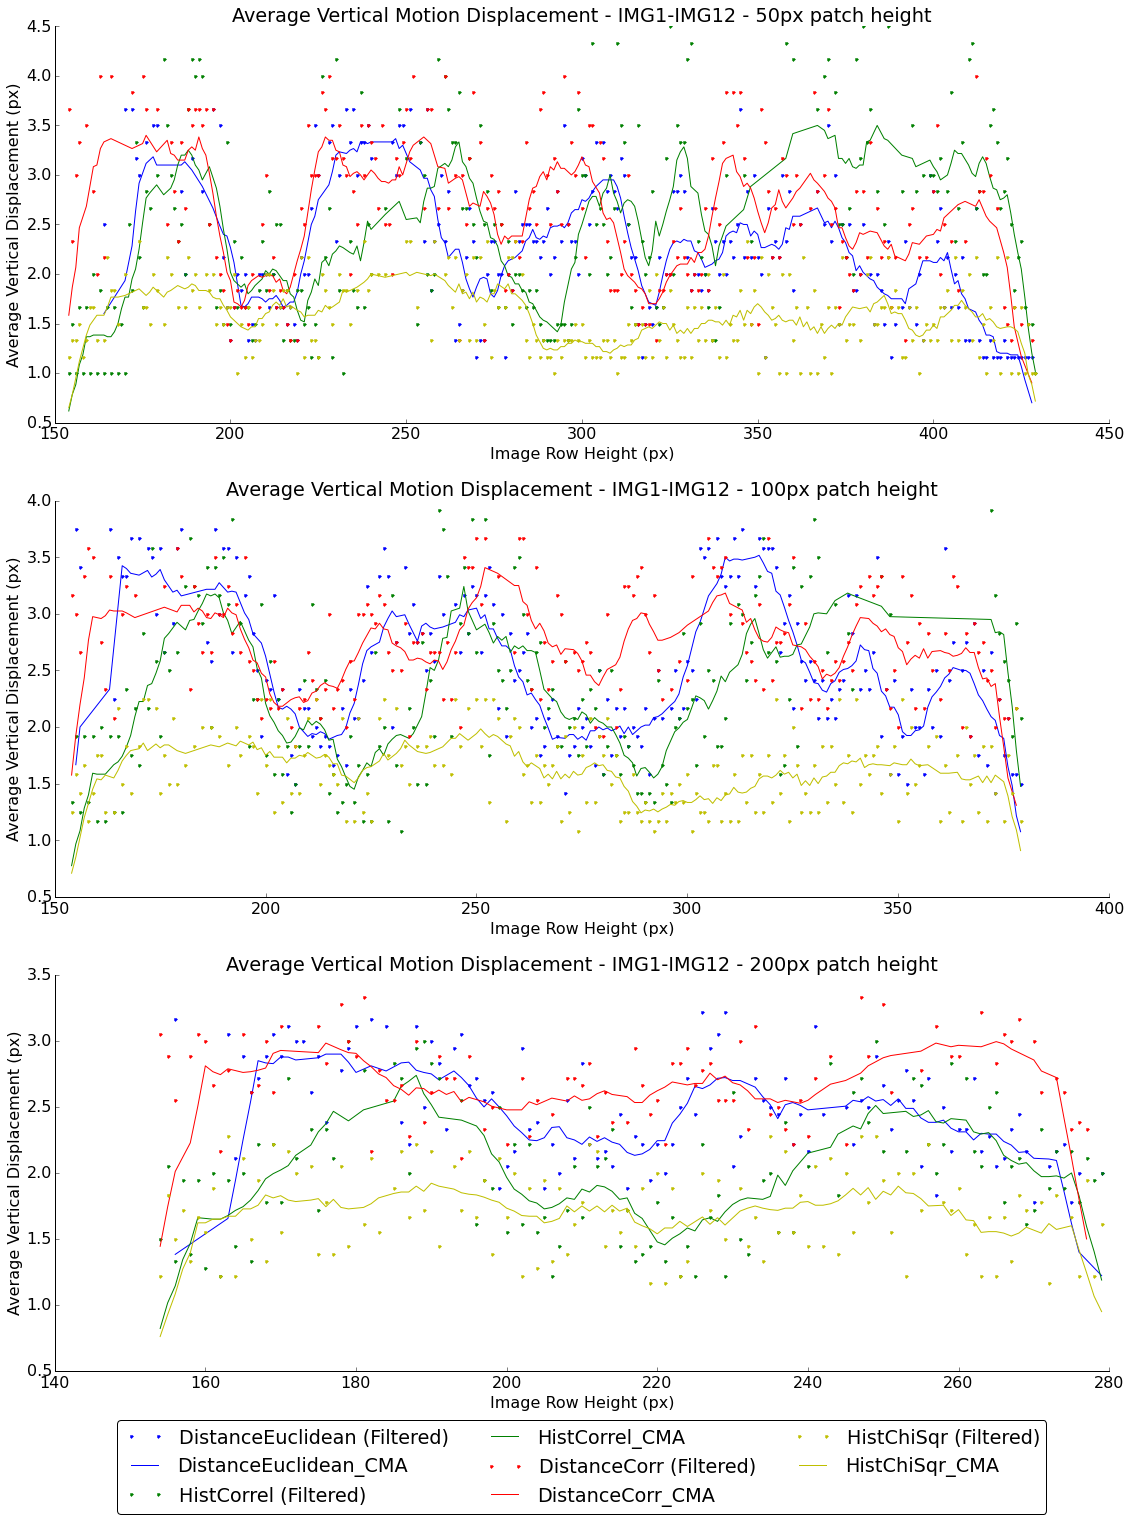
\includegraphics[scale=0.3]{images/results/wiltshire_inside_10cm_scaled}
\caption{Average vertical motion displacement models across all images within ``asian rug" dataset running \textit{non-exhaustive} localised searchwith geometrically scaled template patches. Graph 1 (Top) - Full-width patch with fixed height of 50px; Graph 2 (Middle) Full-width patch with fixed height of 100px; Graph 3 (Bottom) Full-width patch with fixed height of 200px. Solid line indicates centred moving average (10-pixel interval) calculated from filtered results for each appearance-based template matching similarity metric.}
\label{fig:ex3_3_1}
\end{figure}

\clearpage
\begin{figure}[ht!]
\centering
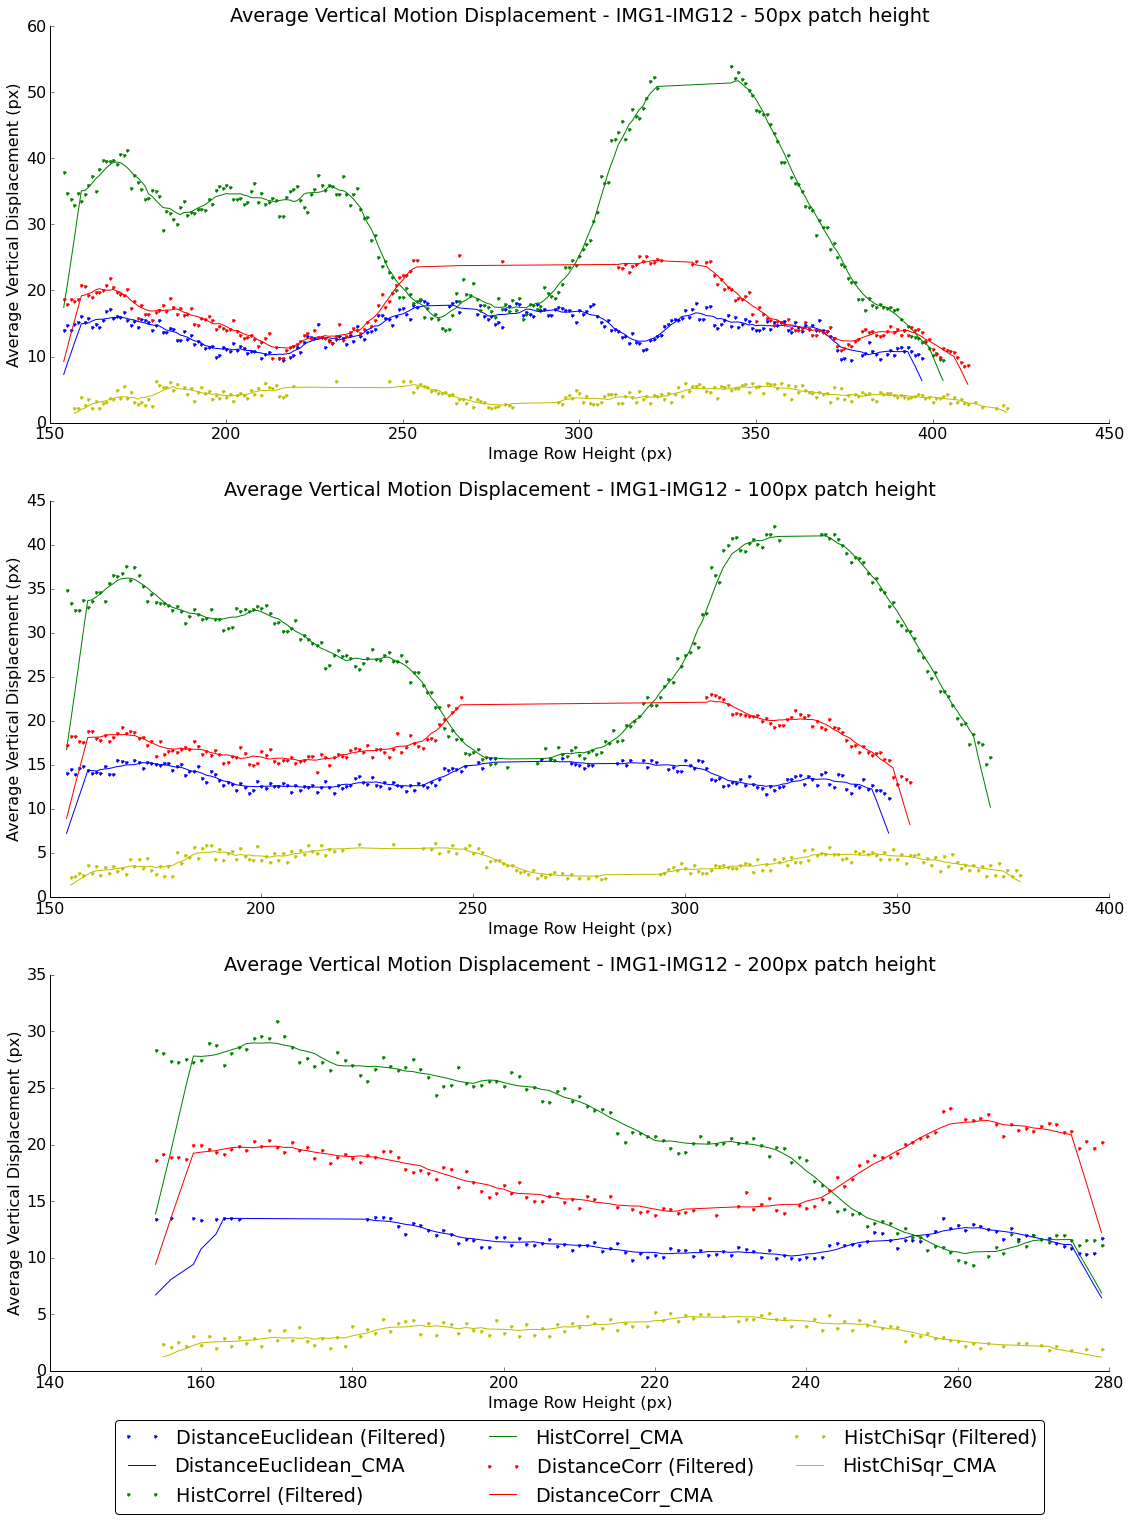
\includegraphics[scale=0.3]{images/results/wiltshire_inside_10cm_scaled_exhaustive}
\caption{Average vertical motion displacement models across all images within ``asian rug" dataset running \textit{exhaustive} localised search with geometrically scaled template patches. Graph 1 (Top) - Full-width patch with fixed height of 50px; Graph 2 (Middle) Full-width patch with fixed height of 100px; Graph 3 (Bottom) Full-width patch with fixed height of 200px. Solid line indicates centred moving average (10-pixel interval) calculated from filtered results for each appearance-based template matching similarity metric.}
\label{fig:ex3_3_2}
\end{figure}

As observed in the experiment two results for dataset three (Figure \ref{fig:ex2_3_1}), the non-exhaustive search (Figure \ref{fig:ex3_3_1}) appear to consist predominantly of noise, and with no correlation. Within the exhaustive search results (Figure \ref{fig:ex3_3_2}), the different categories of similarity measure appear to at times, demonstrate opposite correlation behaviours. In the particular case of the 200px patch-height test (Graph 3), the histogram-based Correlation metric shows an overall negative correlation, while the two distance-based metrics demonstrate a weak positive correlation.

\clearpage
\subsubsection{Dataset 4: Slate Footpath (Outdoors)}

\begin{figure}[ht!]
\centering
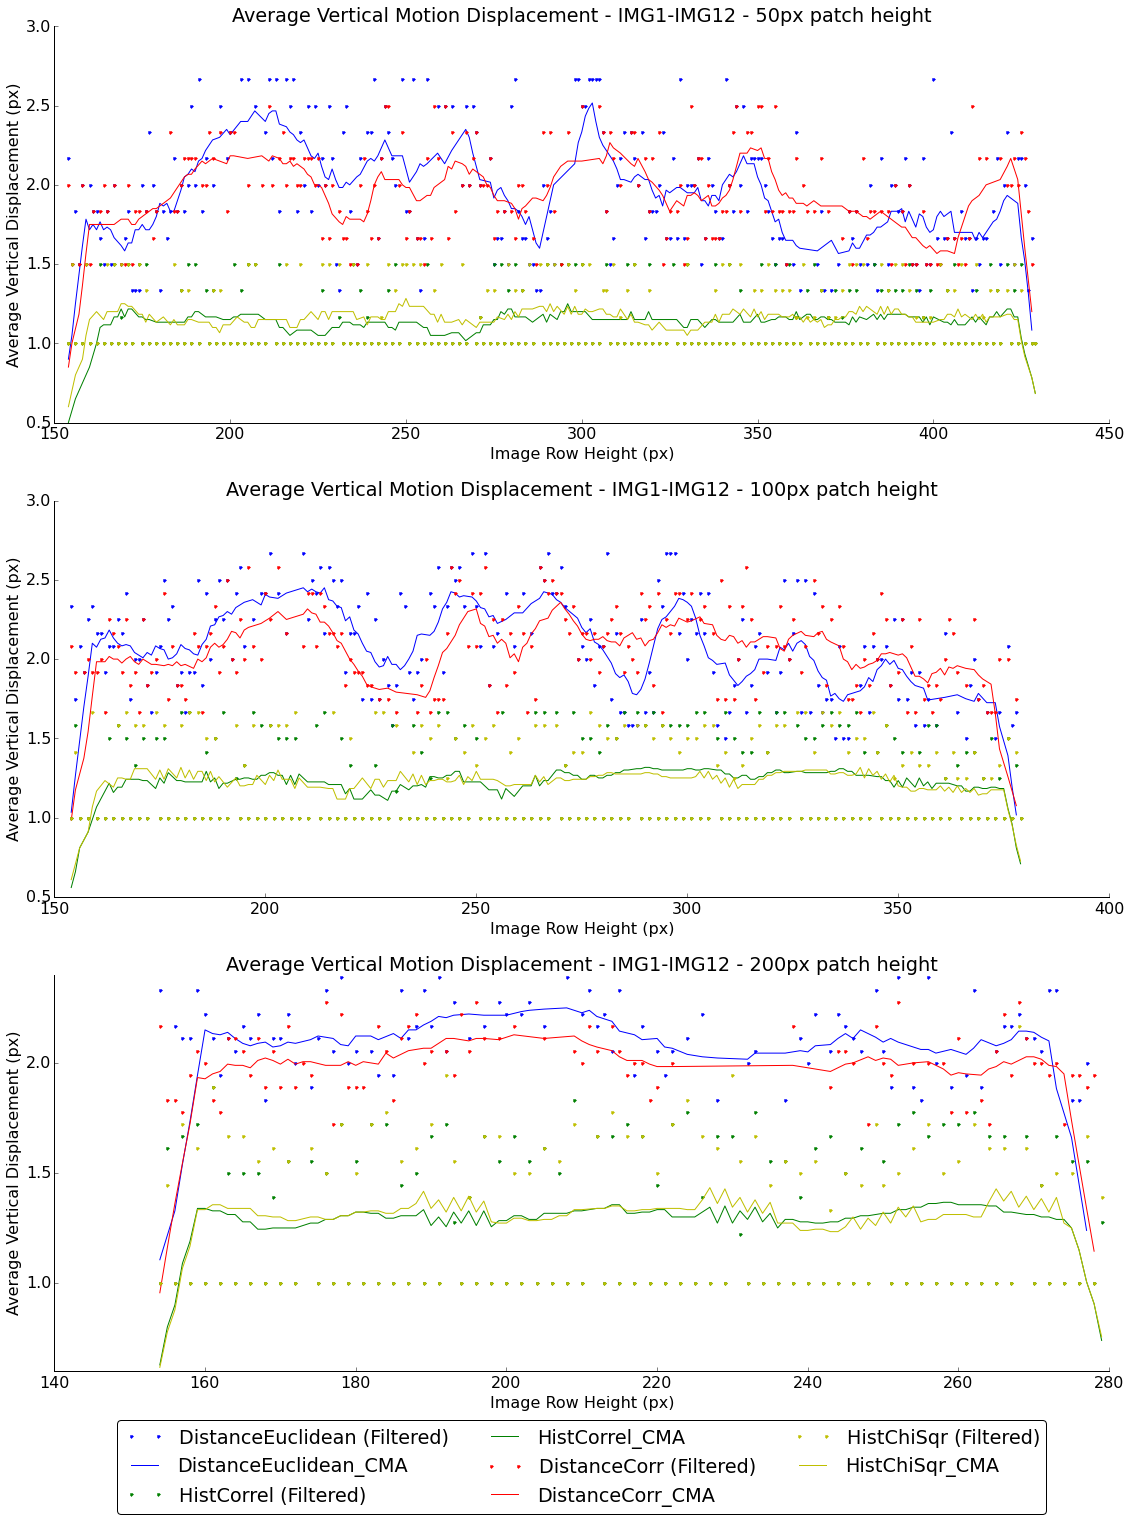
\includegraphics[scale=0.3]{images/results/path_outside_10cm_scaled}
\caption{Average vertical motion displacement models across all images within ``slate footpath" dataset running \textit{non-exhaustive} localised search with geometrically scaled template patches. Graph 1 (Top) - Full-width patch with fixed height of 50px; Graph 2 (Middle) Full-width patch with fixed height of 100px; Graph 3 (Bottom) Full-width patch with fixed height of 200px. Solid line indicates centred moving average (10-pixel interval) calculated from filtered results for each appearance-based template matching similarity metric.}
\label{fig:ex3_4_1}
\end{figure}

\clearpage
\begin{figure}[ht!]
\centering
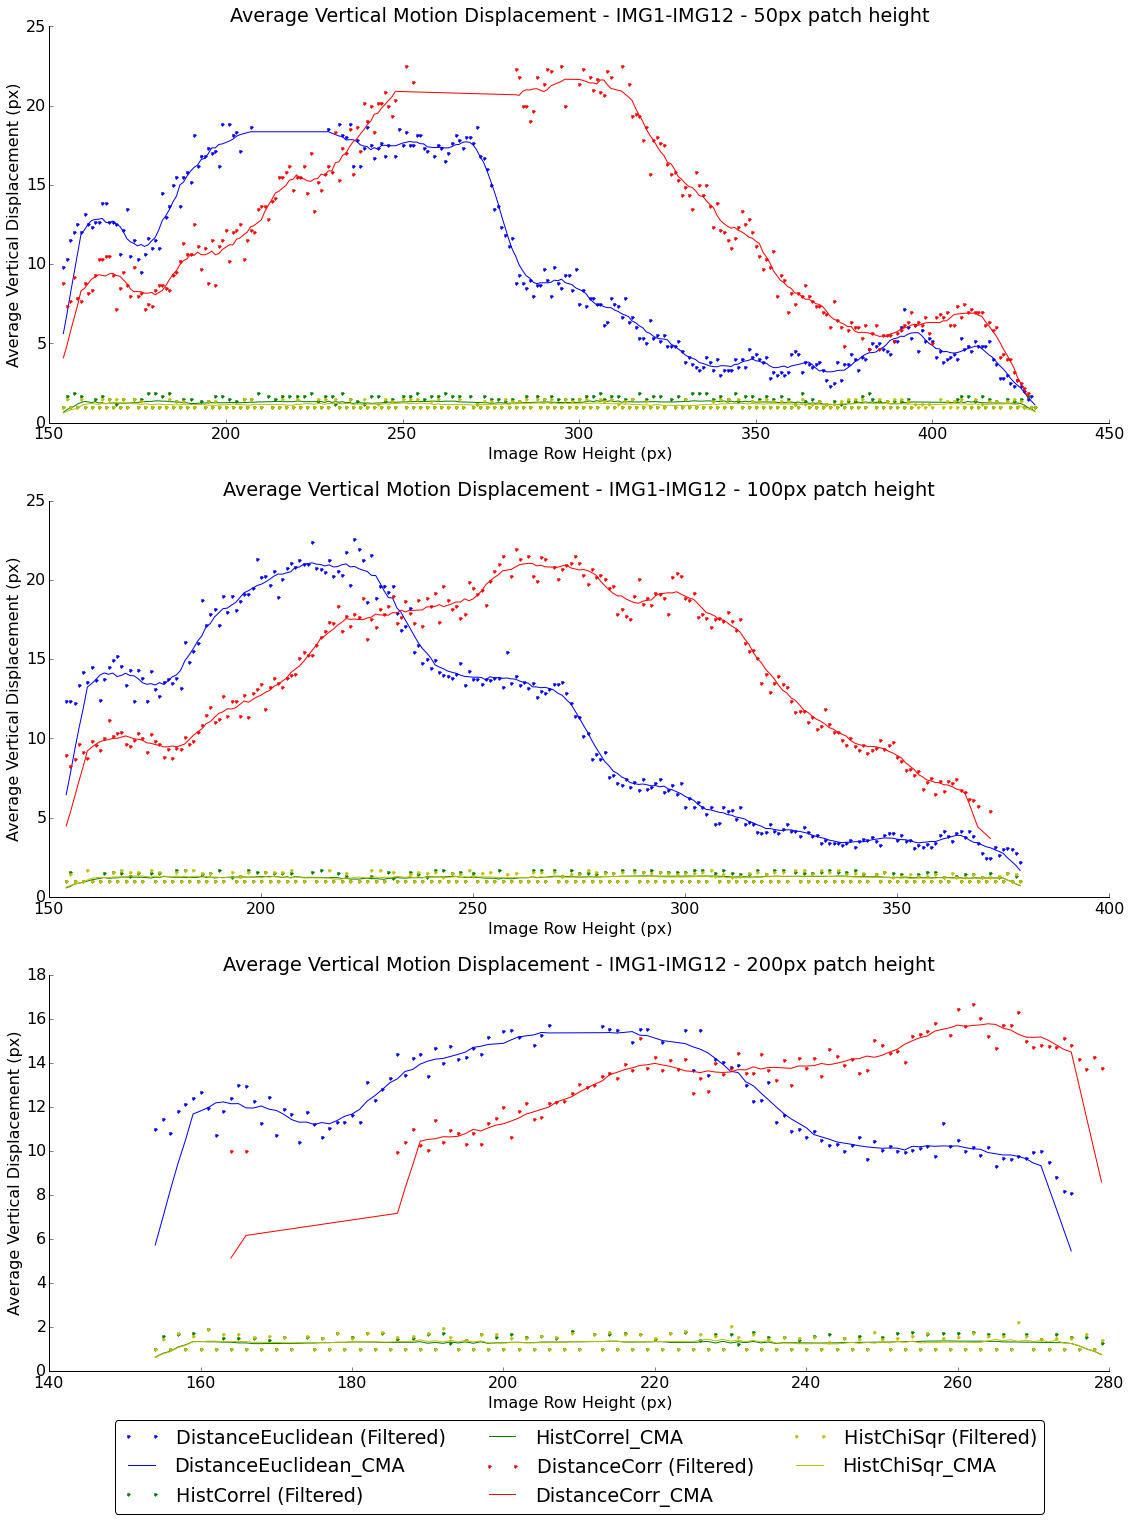
\includegraphics[scale=0.3]{images/results/path_outside_10cm_scaled_exhaustive}
\caption{Average vertical motion displacement models across all images within ``slate footpath" dataset running \textit{exhaustive} localised search with geometrically scaled template patches. Graph 1 (Top) - Full-width patch with fixed height of 50px; Graph 2 (Middle) Full-width patch with fixed height of 100px; Graph 3 (Bottom) Full-width patch with fixed height of 200px. Solid line indicates centred moving average (10-pixel interval) calculated from filtered results for each appearance-based template matching similarity metric.}
\label{fig:ex3_4_2}
\end{figure}

The results for dataset four show that for the non-exhaustive tests (Figure \ref{fig:ex3_4_1}), all of the similarity measures demonstrate significant of levels of noise, with the two distance-based metrics showing a greater level of variability in the results than the two histogram-based metrics. Within the exhaustive results (Figure \ref{fig:ex3_4_2}), a clear performance difference between the two categories of similarity measure is apparent, with the Normalised Cross-Correlation metric showing better overall correlation behaviour than the Euclidean Distance.


\clearpage
\section{Discussion of Results}

Across all three experiments and within all four datasets tested, the results obtained appear to be mixed in terms of the producing the expected performance, however the relative successes and failures of each experiment can be decomposed into a number of different aspects.

\subsection{Fixed Dimension of Patches}

The first of these aspects to consider is the variety of patch sizes, these have remained consistent for each experiment and dataset. 

In terms of robustness to noise, it was the 200px patch size that demonstrated the best overall resilience, in its results caused by erratic matching of incorrect corresponding patches. This is particularly visible in Figures \ref{fig:ex3_4_1}, \ref{fig:ex2_2_2} and \ref{fig:ex2_3_2}, where it is possible to observe a clear smoothing of the results between the 50px and 100px patch sizes, and those of the 200px patch size. Overall it is the 50px patch size that demonstrates the greatest level of noise in results across all experiments. This is most likely caused by the patch size being too small, resulting in the patch failing to extract a large enough region within the image from which it is possible to identify at least one unique feature that can be used to subsequently locate the same unique feature within the second image. At a patch size of 100px, the results obtained indicate a general level of noise that falls between the two extremities observed in the 50px and 200px patch sizes. 

While the results for the 200px patch size may be less prone to noise, they do also indicate a lack of sensitivity to observed vertical displacement. As can be seen in Figures \ref{fig:ex2_2_1}, \ref{fig:ex2_2_2}, \ref{fig:ex3_2_1}, \ref{fig:ex3_2_2} and \ref{fig:ex3_4_1}, while a level of vertical displacement continues to be recorded for the 200px patch size (Graph 3), when compared to the 50px and 100px patch sizes, the level of recorded displacement appears to remain almost constant across all rows within the image. This behaviour would not be expected, and does appear to be isolated to the use of the 200px patch size. The most likely cause is the patch size extracts a template region covering too large an area of the image scene, resulting in little variability of displacement being identified on account of the images only ever showing a relatively small level of motion change between each other. 

It should be noted that this behaviour only appears to begin following the introduction of full-width patches within experiments two and three, and in the results for experiment one, the 200px patch size does appear to show much similar behaviour as the other two patch sizes (Figures \ref{fig:ex1_1_1}, \ref{fig:ex1_1_2}). For both the 50px and 100px patch sizes, a much greater level of sensitivity is generally demonstrated, with the 50px patch showing the largest sensitivity to variations in pixel displacement. While clearly some sensitively is required in order to establish a correlation between the image row and vertical displacement, too much has been shown to cause erratic results.

Overall a patch size of 100px (fixed height of 100px for experiments two and three) appears to provide the best compromise between the reduction of noise and sensitivity to displacement.

\subsection{Appearance-Based Similarity Matching Measures}

When evaluating the four appearance-based similarity measures, the results indicate that the performance of a specific measure can vary significantly in relation to both \textit{itself}, and the relative performance of alternative measures, across the various tests conducted within all experiments. 

A common observation seen throughout all of the results, was the noticeable decline in vertical displacement recorded towards the maximum row height along the X axis. This was expected, and caused by the relationship between search focus on rows towards the bottom of the image, and the decreasing height of the available search window. As a result, the maximum potential displacement that could be recorded also decreases, with the likelihood that patches towards the very bottom of the image will never find a true match as the corresponding features will have since moved below the vertical field of view of the camera. 

In an example from the experiment one results, it can be seen that while the Euclidean Distance (distance-based) measure appears to perform very well across the brightly coloured `spot' carpet within the first dataset (Figure \ref{fig:ex1_1_1} Graph 2), it then suffers a clear decline in performance across the next two datasets, both of which feature \textit{heavily textured terrain} (brick-paved road (dataset two) and asian rug (dataset three)) (Figures \ref{fig:ex1_1_2} and \ref{fig:ex1_1_4}). 

This observation of the poor performance of Euclidean Distance in relation to the histogram-based metrics within datasets containing a high level of texture, is indicative of the differences in approach that each metric demonstrates in determining image similarity. For the two histogram-based metrics, the similarity between two image patches is measured at a \textit{global} level, which in this case is the overall frequency and distribution of colour within both images. 

As a consequence, all of the image `noise' that may have existed originally (\textit{including examples of detailed textures}), subsequently becomes lost. Therefore, when comparing the similarity between two colour histograms, all of the finite detail contained within the original image is in effect ignored, thus leading to an increased chance of finding at least some kind of match, even if this subsequently this match is not accurate. 

In contrast to this, distance-based measures such as the Euclidean Distance retain the finite detail when comparing the similarity between two images. This allows for a greater level of sensitivity and thus potentially better accuracy, but can also result in a failure to identify a correct match due to an acute misalignment of features within the two patches.

While Normalised Cross-Correlation is a distance-based metric, it appears to perform remarkably similar to the Histogram Correlation metric when tested under the same ``heavy texture" terrain conditions as the Euclidean distance (Figures \ref{fig:ex1_1_2} and \ref{fig:ex1_1_4}). The most likely cause for this is due to the normalisation step, whereby a considerable proportion of the finer detail within the original image is potentially lost as a consequence of equalising the range in pixel values can lie. 

Within the final dataset for experiment one (Figure \ref{fig:ex1_1_4}), there was a clear difference in the level of recorded displacement between the histogram-based and distance-based similarity measures. In this situation, the poor performance demonstrated by the two distance-based approaches can be attributed to a lack of distinct features available within the dataset, as a result of the terrain consisting almost exclusively of uniform slate tiles.

\subsection{Exhaustive vs Non-Exhaustive Search}

As part of an enquiry conducted following the end of experiment one into establishing potential causes for the significant reduction in performance observed between the results for dataset one, and the remaining datasets, it was predicted that a most likely partial cause was attributed to an unintended consequence of adopting a \textit{non-exhaustive} approach to searching for matching image patches, as discussed further in Section \ref{searching}. For experiments two and three, additional tests were conducted in order to confirm if any performance gains could be observed between adopting an \textit{exhaustive} vs. \textit{non-exhaustive} search approach. 

Within the tests for experiments two and three, the use of the exhaustive search did appear to provide better overall results in comparison to the non-exhaustive search across all the datasets. While in a selection of cases the gains in the expected performance were significant (Figures \ref{fig:ex2_1_1} vs. \ref{fig:ex2_1_2} and  \ref{fig:ex3_1_1} vs \ref{fig:ex3_1_2}), in the majority of tests exhaustive searching failed to bring about any major improvement in the expected positive correlation behaviour between the image row and recorded vertical displacement. However, it was also observed in these cases that the trend of recorded displacement across the image rows demonstrated behaviour that much less ``sporadic" than in the non-exhaustive results (Figures \ref{fig:ex2_4_1} vs. \ref{fig:ex2_4_2} and  \ref{fig:ex3_3_1} vs \ref{fig:ex3_3_2}).

An additional observation from the comparison of results between the exhaustive and non-exhaustive searches highlighted how in a large proportion of cases, the increase in performance for the \textit{distance-based} similarity measures far outweighed the level of improvement demonstrated by the \textit{histogram-based} measures (Figures). Given that in these cases all four similarity measures were tested under the same relative conditions (i.e. all were tested together under either a non-exhaustive or exhaustive search), the most likely explanation for these significant differences in performance gain is simply that under those specific conditions (i.e. current dataset, patch size etc.) the distance-based similarity measures genuinely were able to perform better than the histogram-based measures, but in the results for the non-exhaustive search, this observation was in fact ``masked" for the reasons detailed in Section \ref{searching}.

\subsection{Conclusion of Results}

Following analysis of all the results gathered across the three primary experiments, it is not possible to identify one specific combination of experiment method, patch size and appearance-based similarity metric, that is capable of demonstrating an optimal solution across variations in terrain type.

% in order to generate a vertical displacement model that is able to confirm the predicted positive correlation between the vertical position of a feature within the current scene, and the level of vertical displacement that it demonstrates between two consecutive images.

When exclusively considering the four variations in terrain type selected for use within this investigation, the best solution was provided through the use of geometrically-scaled template patches, evaluated within the method for experiment three.

More specifically, it was found that performing geometric scaling of full-width 100px-high template patches, in conjunction with exhaustive appearance-based template matching using the Euclidean Distance similarity metric, provided the best available example of a well-defined vertical displacement model (Figure \ref{fig:ex3_1_2} (Graph 2)) that accurately demonstrated the behaviour predicted in the hypothesis (see Section \ref{hypo-calib}).

While this particular combination happens to demonstrate the best performance with respect to this specific dataset, there are other instances where this exact same combination would fail to produce such a successful outcome. An example of such an instance can be observed within Figure \ref{fig:ex3_2_2}. This is an observation that appears to be common within a large proportion of the various possible experimental parameters evaluated as part of this study. 

As a result of analysing the experiments, the overarching conclusion to be drawn,is that the results obtain may be regarded as inconclusive. However, while certainly further research is required this investigation and it's results have highlighted that it is unlikely one particular solution will suffice. Therefore, a key focus for any further investigation to develop upon this work, would be to attempt to identify the most appropriate configuration setting for each particular terrain type, thereby hopefully ensuring that the maximum possible accuracy can be obtained, regardless of a robot's surrounding environment. 
  

 
  


\chapter{Critical Evaluation}
%
%Examiners expect to find in your dissertation a section addressing such questions as:
%
%\begin{itemize}
%   \item Were the requirements correctly identified? 
%   \item Were the design decisions correct?
%   \item Could a more suitable set of tools have been chosen?
%   \item How well did the software meet the needs of those who were expecting to use it?
%   \item How well were any other project aims achieved?
%   \item If you were starting again, what would you do differently?
%\end{itemize}
%
%Such material is regarded as an important part of the dissertation; it should demonstrate that you are capable not only of carrying out a piece of work but also of thinking critically about how you did it and how you might have done it better. This is seen as an important part of an honours degree. 
%
%There will be good things and room for improvement with any project. As you write this section, identify and discuss the parts of the work that went well and also consider ways in which the work could be improved. 
%
%Review the discussion on the Evaluation section from the lectures. A recording is available on Blackboard. 

\section{Research Aims}

\section{Technical Achievement}

\section{Project Management}

\section{Conclusion}
% add any additional chapters here

\setemptyheader
\addcontentsline{toc}{chapter}{Appendices}
\chapter*{Appendices}
\pagebreak

% start the appendix - sets up different numbering
\fancypagestyle{plain}{%
%\fancyhf{} % clear all header and footer fields
\fancyhead[L]{\textsl{Appendix\ \thechapter}}
\fancyhead[R]{\textsl{\leftmark}}}

\appendix
\fancyhead[L]{\textsl{Appendix\ \thechapter}}
\fancyhead[R]{\textsl{\leftmark}}
\fancyhead[C]{}
\fancyfoot[C]{\thepage}
\renewcommand{\headrulewidth}{0.4pt}
\renewcommand{\chaptermark}[1]{\markboth{#1}{}}

\fancyhead[L]{\textsl{Appendix\ \thechapter}}
\fancyhead[R]{\textsl{\leftmark}}
\fancyfoot[C]{{\thepage} of \pageref{LastPage}}

% include any appendices here
\chapter{Third-Party Code and Libraries}

If you have made use of any third party code or software libraries, i.e. any code that you have not designed and written yourself, then you must include this appendix. 

As has been said in lectures, it is acceptable and likely that you will make use of third-party code and software libraries. The key requirement is that we understand what is your original work and what work is based on that of other people. 

Therefore, you need to clearly state what you have used and where the original material can be found. Also, if you have made any changes to the original versions, you must explain what you have changed. 

As an example, you might include a definition such as: 

Apache POI library � The project has been used to read and write Microsoft Excel files (XLS) as part of the interaction with the client�s existing system for processing data. Version 3.10-FINAL was used. The library is open source and it is available from the Apache Software Foundation 
\cite{apache_poi}. The library is released using the Apache License 
\cite{apache_license}. This library was used without modification. 

\chapter{Code samples}

%\section{Random Number Generator}
%
%The Bayes Durham Shuffle ensures that the psuedo random numbers used in the simulation are further shuffled, ensuring minimal correlation between subsequent random outputs \cite{NumericalRecipes}.
%
%\begin{verbatim}
% #define IM1 2147483563
% #define IM2 2147483399
% #define AM (1.0/IM1)
% #define IMM1 (IM1-1)
% #define IA1 40014
% #define IA2 40692 
% #define IQ1 53668
% #define IQ2 52774
% #define IR1 12211
% #define IR2 3791
% #define NTAB 32
% #define NDIV (1+IMM1/NTAB)
% #define EPS 1.2e-7
% #define RNMX (1.0 - EPS)
% 
% double ran2(long *idum)
% {
%   /*---------------------------------------------------*/
%   /* Minimum Standard Random Number Generator          */
%   /* Taken from Numerical recipies in C                */
%   /* Based on Park and Miller with Bays Durham Shuffle */
%   /* Coupled Schrage methods for extra periodicity     */
%   /* Always call with negative number to initialise    */
%   /*---------------------------------------------------*/	
% 
%   int j;
%   long k;
%   static long idum2=123456789;
%   static long iy=0;
%   static long iv[NTAB];
%   double temp;
% 
%   if (*idum <=0)
%   {
%     if (-(*idum) < 1)
%     {
%       *idum = 1;
%     }else
%     {
%       *idum = -(*idum);
%     }
%     idum2=(*idum);
%     for (j=NTAB+7;j>=0;j--)
%     {
%       k = (*idum)/IQ1;
%       *idum = IA1 *(*idum-k*IQ1) - IR1*k;
%       if (*idum < 0)
%       {
%         *idum += IM1;
%       }
%       if (j < NTAB)
%       {
%         iv[j] = *idum;
%       }
%     }
%     iy = iv[0];	
%   }
%   k = (*idum)/IQ1;
%   *idum = IA1*(*idum-k*IQ1) - IR1*k;
%   if (*idum < 0)
%   {
%     *idum += IM1;
%   }
%   k = (idum2)/IQ2;
%   idum2 = IA2*(idum2-k*IQ2) - IR2*k;
%   if (idum2 < 0)
%   {
%     idum2 += IM2;
%   }
%   j = iy/NDIV;
%   iy=iv[j] - idum2;
%   iv[j] = *idum;
%   if (iy < 1)
%   {
%     iy += IMM1;
%   }
%   if ((temp=AM*iy) > RNMX)
%   {
%     return RNMX;
%   }else
%   {
%     return temp;	
%   }
% }
% 
%\end{verbatim}
%


\fancypagestyle{plain}{%
   \fancyhead{} %[C]{Annotated Bibliography}
   \fancyfoot[C]{{\thepage} of \pageref{LastPage}} % except the center
   \renewcommand{\headrulewidth}{0pt}
   \renewcommand{\footrulewidth}{0pt}
}

\setemptyheader

\nocite{*} % include everything from the bibliography, irrespective of whether it has been referenced.

% the following line is included so that the bibliography is also shown in the table of contents. There is the possibility that this is added to the previous page for the bibliography. To address this, a newline is added so that it appears on the first page for the bibliography. 
\addcontentsline{toc}{chapter}{Annotated Bibliography} % Adds References to contents page

%
% example of including an annotated bibliography. The current style is an author date one. If you want to change, comment out the line and uncomment the subsequent line. You should also modify the packages included at the top (see the notes earlier in the file) and then trash your aux files and re-run. 
%\bibliographystyle{authordate2annot}
\bibliographystyle{IEEEannot}
\renewcommand{\bibname}{Annotated Bibliography} 
\bibliography{References/references} % References file


\end{document}
